\documentclass[11pt,a4paper]{article}
% https://www.iccat.int/Documents/SCRS/Other/Guide_ColVol_ENG.pdf

\usepackage[margin=2.5cm]{geometry}
\usepackage{setspace}
\usepackage{authblk}
\usepackage{graphicx}
\usepackage{booktabs}
\usepackage{tabularx}
\usepackage{array}
\usepackage{amsmath,amssymb}
\usepackage{hyperref}
\usepackage{natbib}
\usepackage{float}
\hypersetup{hypertexnames=false}

\setstretch{1.0}
\parskip=6pt
\parindent=0pt
\pagestyle{empty}
\setlength{\emergencystretch}{2em}

% ---------- Title & authors (fixed for reuse) ----------
\title{\textbf{Three Intertwined Strands: Internal, External, and Robustness Diagnostics for Integrated Stock Assessments}}

\author[1]{Laurence T. Kell}
\author[2]{Massimiliano Cardinale}

\affil[1]{Centre for Environmental Policy, Imperial College London, Weeks Building,
16--18 Princes Gardens, London, SW7 1NE, UK}
\affil[2]{Swedish University of Agricultural Sciences, Department of Aquatic Resources,
Institute of Marine Research, SE-453 30 Lysekil, Sweden}

\date{} % no date in SCRS docs (footnote on title carries disclaimer)

\begin{document}
\maketitle

% ---------- SUMMARY ----------
\begin{center}
\textit{SUMMARY}
\end{center}

Integrated stock assessments are often judged based on convergence, fit to data, and the precision of management quantities. These checks are necessary but not sufficient for the provision of robust scientific advice. This paper organises assessment diagnostics into three intertwined strands: \textbf{internal} diagnostics, which test consistency with the model likelihood and fitted data; \textbf{external} diagnostics, which test consistency with specified evidence outside the likelihood; and \textbf{robustness} diagnostics, which test whether advice is stable under pre-specified alternative structures. The main body sets out the framework and illustrates it with selected Stock Synthesis (SS3) shortfin mako examples; the appendices provide reproducible templates for detailed diagnostics, plots, tables, and code outputs. To ensure best practice, we recommend routine three-strand reporting: a minimum diagnostic checklist for accepted runs and key sensitivities, explicit separation of verification, validation, uncertainty and sensitivity, and rebuilding-based diagnostics for non-retained bycatch species where achieving high catch rates in the long term is not the primary management objective.

\vspace{1ex}

\textbf{KEYWORDS}

Stock assessment, Stock Synthesis, diagnostics, validation, robustness, shortfin mako.

\newpage
\tableofcontents
\newpage

% ---------- MAIN TEXT ----------
\section{Introduction}

Scientific fishery advice depends on model outputs that are latent, i.e. seldom observed directly, such as spawning biomass, recruitment and fishing mortality. It also depends on biological reference points that are commonly derived from equilibrium-based production functions. Stock Synthesis (SS3) \citep{MethotWetzel2013}, for example, provides a transparent and flexible framework for combining catch, abundance indices, composition data, and biological assumptions. That flexibility increases the need for diagnostics that distinguish between a technically well-fitted model and a model that is robust and adequate for management advice.

Diagnostics can be summarised by three intertwined strands. \textbf{Internal} diagnostics evaluate whether the fitted model is consistent with its own assumptions, likelihood components, and data inputs. \textbf{External} diagnostics ask whether model outputs are biologically and empirically plausible; here ``plausible'' means consistent with specified evidence outside the fitted likelihood, such as life history, fishery-independent surveys, fishery behaviour, environmental drivers, and spatial information. \textbf{Robustness} diagnostics ask whether conclusions and advice are stable under alternative assumptions, including different stock--recruitment forms, natural mortality or selectivity, data weighting, process-error assumptions, retrospective peels, and hindcasts.

The framework draws on diagnostic tools and guidance developed in R and in assessment practice, including the diagnostic ``cookbook'' of \citet{carvalho2021cookbook}, empirical validation and hindcasting \citep{kell2016evaluation,kell2024empirical}, and recent reference-point evaluation guidance \citep{ICES2024}. The distinction is practical: a model may converge, fit the main index, and produce biomass trends consistent with external evidence, while scale remains poorly informed by data and reference points depend strongly on fixed values, priors, data weighting, or the treatment of process error.

This paper shows how the three-strand framework can be applied using shortfin mako shark SS3 scenarios \citep{ICCAT2025SMA}. The scenarios were not adopted for advice and are used only to demonstrate how diagnostic classes can be reported in a working group setting. The main text is therefore intentionally selective: it describes the review framework, gives a small number of decision-relevant examples, and leaves the full diagnostic workflow to the appendices. This structure allows the SCRS paper to be submitted as a coherent framework paper while retaining space to update the technical diagnostics as generic R functions and case-study scripts are refined.

\section{Diagnostic Framework}

\subsection{Internal Diagnostics}

Internal diagnostics test whether the fitted assessment is consistent with the likelihood, parameterisation, and assumptions used by the model. For an SS3 assessment this includes convergence status, maximum gradient, Hessian behaviour, parameters near bounds, influential correlations, likelihood-component contributions, residual diagnostics for indices and compositions, effective sample sizes, recruitment deviations, and information content for key quantities.

For management advice, the most important internal question is not simply whether the model converged, but whether management quantities are informed by data. Examples include whether steepness, natural mortality, selectivity, or survey catchability are estimated, fixed, penalised, or effectively determined by bounds and priors. Where MSY-based quantities are derived from a stock--recruitment relationship, internal diagnostics should ask whether the relevant contrast in spawning biomass and recruitment exists, whether residuals are independent and stationary, and whether likelihood profiles show information in the data rather than only in model assumptions \citep{kell2025profile}.

Internal diagnostics should also distinguish \textbf{identifiability}, \textbf{estimability}, and \textbf{regularisation}. Identifiability asks whether different parameter combinations can produce the same model output, for example when productivity, natural mortality, selectivity, and growth combine to give similar production dynamics. Estimability asks whether the available data provide enough contrast to estimate a parameter precisely, even when the model structure is identifiable. Likelihood profiling and Hessian diagnostics can disclose parameter confounding, ill-conditioned models, and cases where uncertainty intervals from the Hessian and profile disagree \citep{kell2025profile}. Where instability is detected, regularised Bayesian methods such as MCMC with \texttt{adnuts} provide a practical route to stabilise poorly informed parameters, reformulate selectivity or other weakly estimated terms, and obtain within-model uncertainty for derived quantities \citep{courtney2024adnuts}. The North Atlantic blue shark example shows that this workflow is especially relevant for data-limited SS3 assessments where convergence alone does not show whether advice-relevant quantities are well determined.

\subsection{External Diagnostics}

External diagnostics compare model behaviour with evidence outside the fitted likelihood. This includes consistency with life-history knowledge, consistency of growth and maturity with biological knowledge, coherence between biomass trends and survey perceptions, evidence-consistent exploitation history, age-structure signals, spatial and environmental information, and agreement with independent or pre-standardised data products. This provides an explicit definition of plausibility for review purposes.

External diagnostics are especially important when a model uses standardised survey indices or pre-processed composition data. If environmental effects have already been absorbed in a spatially explicit model such as VAST, sdmTMB, or comparable standardisation model, then adding similar covariates inside SS3 may double-count the signal. Conversely, if spatial availability or changes in vulnerability are not represented in the assessment, recruitment deviations, selectivity deviations, or process-error signals may absorb effects that are not recruitment processes. External diagnostics therefore ask whether the assessment is biologically credible, not only statistically well fitted.

\subsection{Robustness Diagnostics}

Robustness diagnostics evaluate whether stock status, reference points, and advice are stable under pre-specified alternative structures. They include retrospective analyses, hindcasts and prediction skill, likelihood profiles, alternative stock--recruitment forms, data-weighting sensitivities, alternative natural mortality or selectivity structures, and scenario or ensemble analyses. Robustness diagnostics are linked to validation because a model adequate for advice should have useful prediction skill over the time horizons used for management \citep{kell2016evaluation,kell2024empirical}.

In practice, robustness separates uncertainty conditional on one model from sensitivity across pre-specified models. Confidence intervals from a single accepted run describe estimation uncertainty conditional on that run. Differences among acceptable scenarios describe structural uncertainty. For advice, both matter. If alternative structures produce similar historical biomass trajectories but different $B_{\mathrm{MSY}}$, $F_{\mathrm{MSY}}$, or catch limits, then the assessment may be adequate for tracking status while being less reliable for precise MSY-based advice.

Robustness diagnostics should also distinguish between \textbf{tail probabilities} and \textbf{central tendencies}. Limit reference points are primarily risk statements, so diagnostics should report probabilities of undesirable events, for example $P(B < B_{\mathrm{lim}})$, $P(F > F_{\mathrm{lim}})$, or the probability of falling below a biomass threshold during a projection period \citep{Roux2022,Fischer2023}. Target reference points are usually interpreted through central tendencies, such as the median or mean of $B/B_{\mathrm{MSY}}$, $F/F_{\mathrm{MSY}}$, catch, or rebuilding time, together with their spread. A scenario may have an acceptable median trajectory but an unacceptable lower tail, or similar median status but very different probabilities of breaching a limit. Limits may be informed by only one assessment in a set of scenarios or ensemble while medians by all. Robustness reporting should therefore show both: central tendencies for targets and tail probabilities for limits.

\begin{table}[H]
  \centering
  \caption{Three diagnostic classes and their role in assessment review.}
  \label{tab:diag-classes}
  \small
  \begin{tabularx}{\textwidth}{>{\raggedright\arraybackslash}p{3.0cm}>{\raggedright\arraybackslash}p{5.0cm}>{\raggedright\arraybackslash}X}
    \toprule
    Diagnostic class & Main question & Examples for SS3 assessments \\
    \midrule
    Internal & Is the model consistent with its likelihood, assumptions, and fitted data? & Convergence, gradients, Hessian status, residuals, effective sample size, recruitment deviations, likelihood profiles, parameters near bounds. \\
    External & Is model behaviour consistent with evidence outside the likelihood? & Life history, survey perception, age structure, spatial and environmental consistency, biological evidence for productivity and mortality. \\
    Robustness & Would conclusions and advice change under pre-specified alternative structures? & Retrospectives, hindcasts, stock--recruitment alternatives, data weighting, natural mortality and selectivity. \\
    \bottomrule
  \end{tabularx}
\end{table}

Table~\ref{tab:diag-classes} summarises the three strands as a practical review checklist. The strands also map onto familiar review concepts: internal diagnostics support \textbf{verification} of implementation and fit; external diagnostics and hindcasts support \textbf{validation} against information not used directly in fitting; and robustness diagnostics separate \textbf{uncertainty} within a model from \textbf{sensitivity} across model structures.

\section{Scope}

The diagnostics described here are available as reproducible R workflows, but not all diagnostics are currently available in one package. The workflow uses \texttt{r4ss}, \texttt{ss3diags}, \texttt{ss3om}, \texttt{FLCore}, \texttt{sstruth}, \texttt{FLRebuild} and \texttt{kobe}.

\texttt{r4ss} reads in \texttt{SS3} inputs and outputs into \texttt{R} lists, data frames, and matrices, \texttt{ss3om} converts these to \texttt{FLR} and \texttt{FLCore} objects that represent stocks, stock recruitment relationships, production functions, biological reference points, length frequency distributions and other inputs, estimates and derived quantities. \texttt{ss3diags} implements common diagnostics based on the cookbook. While \texttt{sstruth} creates operating model and other tools for simulation testing, and \texttt{FLRebuild} implements a variety of reference points, \texttt{kobe} provides stock estimates used for management advice. \texttt{FLR} and \texttt{FLCore} are generic and can be used for any stock assessment, i.e. helping to compare and combine model frameworks.


\begin{table}[H]
  \centering
  \caption{Diagnostic workflows and main package dependencies.}
  \label{tab:diag-availability}
  \scriptsize
  \begin{tabularx}{\textwidth}{>{\raggedright\arraybackslash}p{3.0cm}>{\raggedright\arraybackslash}X>{\raggedright\arraybackslash}p{4.2cm}}
    \toprule
    Diagnostic workflow & Model scope & Main packages \\
    \midrule
    SS3 fit and residual diagnostics & SS3-specific because it reads SS3 report objects through \texttt{r4ss}; concepts also apply to other integrated models if equivalent residuals and retrospective outputs are available. & \texttt{r4ss}, \texttt{ss3diags} \\
    Retrospectives and hindcasts & Implementation is strongest for SS3; the diagnostic idea is model-class agnostic and applies to any assessment that can be re-run with terminal years removed and forecasts compared with withheld data. & \texttt{r4ss}, \texttt{ss3diags}, \texttt{sstruth} \\
    Process-error and production-function diagnostics & The SMA implementation reads SS3 scenarios, but the diagnostic is not SS3-specific. It requires biomass, removals, reference points, and an implied or explicit production function. For biomass-dynamic models such as JABBA or SPiCT the production function is explicit; for SS3 it is reconstructed from age-structured output. & \texttt{ss3om}, \texttt{sstruth}, \texttt{FLCore}, \texttt{FLRebuild} \\
    Likelihood profiles and identifiability & Examples are SS3/r4ss-specific, but likelihood profiling and Hessian diagnostics are relevant to any likelihood-based assessment framework. & \texttt{r4ss}; assessment model executable \\
    Stock--recruitment and reference-point robustness & The implemented bridge is SS3/yellowfin-specific, but testing alternative stock--recruitment forms, steepness, and proxy reference points is relevant to all age-structured assessments. & \texttt{r4ss}, \texttt{ss3om}, \texttt{FLCore}, \texttt{FLBRP}, \texttt{FLRebuild} \\
    MVLN status and advice uncertainty & Implemented for SS3 covariance and derived quantities, but the idea applies to any model that provides a covariance matrix or posterior/Monte Carlo draws for stock status and reference points. & \texttt{r4ss}, \texttt{kobe}, \texttt{FLCore} \\
    External biological checks & Not model-specific. These checks require life-history, survey, fishery, and spatial/ecological information outside the fitted likelihood. & \texttt{FLCore}, \texttt{ggplot2}, assessment-specific data packages \\
    \bottomrule
  \end{tabularx}
\end{table}

Both stock--recruitment relationships and production functions are essentially model-derived, or emergent, properties rather than directly observed biological laws. In SS3, annual recruitment deviations are estimable quantities within the age-structured likelihood, and they absorb deviations from the assumed stock--recruitment relationship as well as effects of misspecified mortality, selectivity, catchability, or productivity. In state-space biomass-dynamic models, by contrast, process-error deviations are usually explicit deviations in the biomass state equation. Models such as JABBA and SPiCT estimate the production function directly, for example through parameters controlling productivity, carrying capacity and shape, whereas in SS3 the equivalent production function is implicit: it is derived from yield-per-recruit, spawning-biomass-per-recruit, selectivity, life-history parameters, and the stock--recruitment relationship. A main distinction is therefore not whether a production function exists, but whether it is parameterised explicitly and estimated during fitting, or is an implicit consequence of the fitted age-structured model and derived post hoc for diagnostic interpretation. SS3 recruitment deviates can therefore also be mapped to process error. 

The diagnostic \textit{classes} are not specific to SS3 or to age-structured models. Internal, external, and robustness diagnostics are general assessment-review concepts. The current code base is strongest for SS3 because \texttt{r4ss} and \texttt{ss3diags} provide a set of diagnostics, summaries, and plotting functions that have been widely used. Biomass-dynamic models such as JABBA and SPiCT can use the same diagnostic strands, but the implementation changes: internal checks use posterior or state-space residuals, process error is an explicit biomass-state deviation, and production functions are estimated directly rather than reconstructed from age-structured outputs. For an empirical management procedure, internal diagnostics might check that the indicator and control rule are implemented correctly, external diagnostics might compare the indicator with independent survey or spatial information, and robustness diagnostics would be evaluated through simulation testing. Empirical and data-limited methods may have fewer internal likelihood diagnostics and rely more on simulation, hindcasting where possible, and management-procedure testing.

\section{Illustrative Examples from SS3 Shortfin Mako Scenarios}

\subsection{Scope of the Examples}

The illustrative examples use the SS3 scenarios developed during the 2025 ICCAT shortfin mako shark assessment meeting and analysed in \citep{ICCAT2025SMA}. They are not intended to reproduce every diagnostic output. Instead, they show how a small set of plots can carry the main message of each diagnostic strand in the body of an SCRS paper: internal diagnostics reveal production-function and residual behaviour; external diagnostics identify age-structure and biomass-currency issues; and robustness diagnostics show why reference points and rebuilding conclusions should be treated as conditional. The scenarios were used to derive time series of spawning stock biomass, harvest intensity, production-function, MSY-scaled, and process-error diagnostics from SS3 outputs extracted using \texttt{r4ss}. Surplus production and process residuals were then calculated from the SS3-derived biomass and catch series \citep{walters2008surplus}.

The shortfin mako stock has strong age-structure effects, catches are dominated by juveniles and subadults, although management quantities are expressed on a spawning-biomass scale. As a result, apparent production dynamics can be affected by the mismatch between the reproductive state variable and the age classes removed by fishing \citep{winker2020age}. This makes the case study a useful stress test for separating internal fit, external biological consistency, and robustness of management interpretation.

\subsection{Internal Diagnostics in the Case Study}
The first internal diagnostic question is whether the estimated trajectory and implied production function are compatible with the model assumptions. SS3 outputs were converted into MSY-scaled time series and phase plots. The time-series diagnostics show that catch tracks fishing intensity more closely than spawning biomass, while the production phase plots show that realised surplus production does not always align with the equilibrium production curves implied by reference points.

\begin{figure}[H]
  \centering
  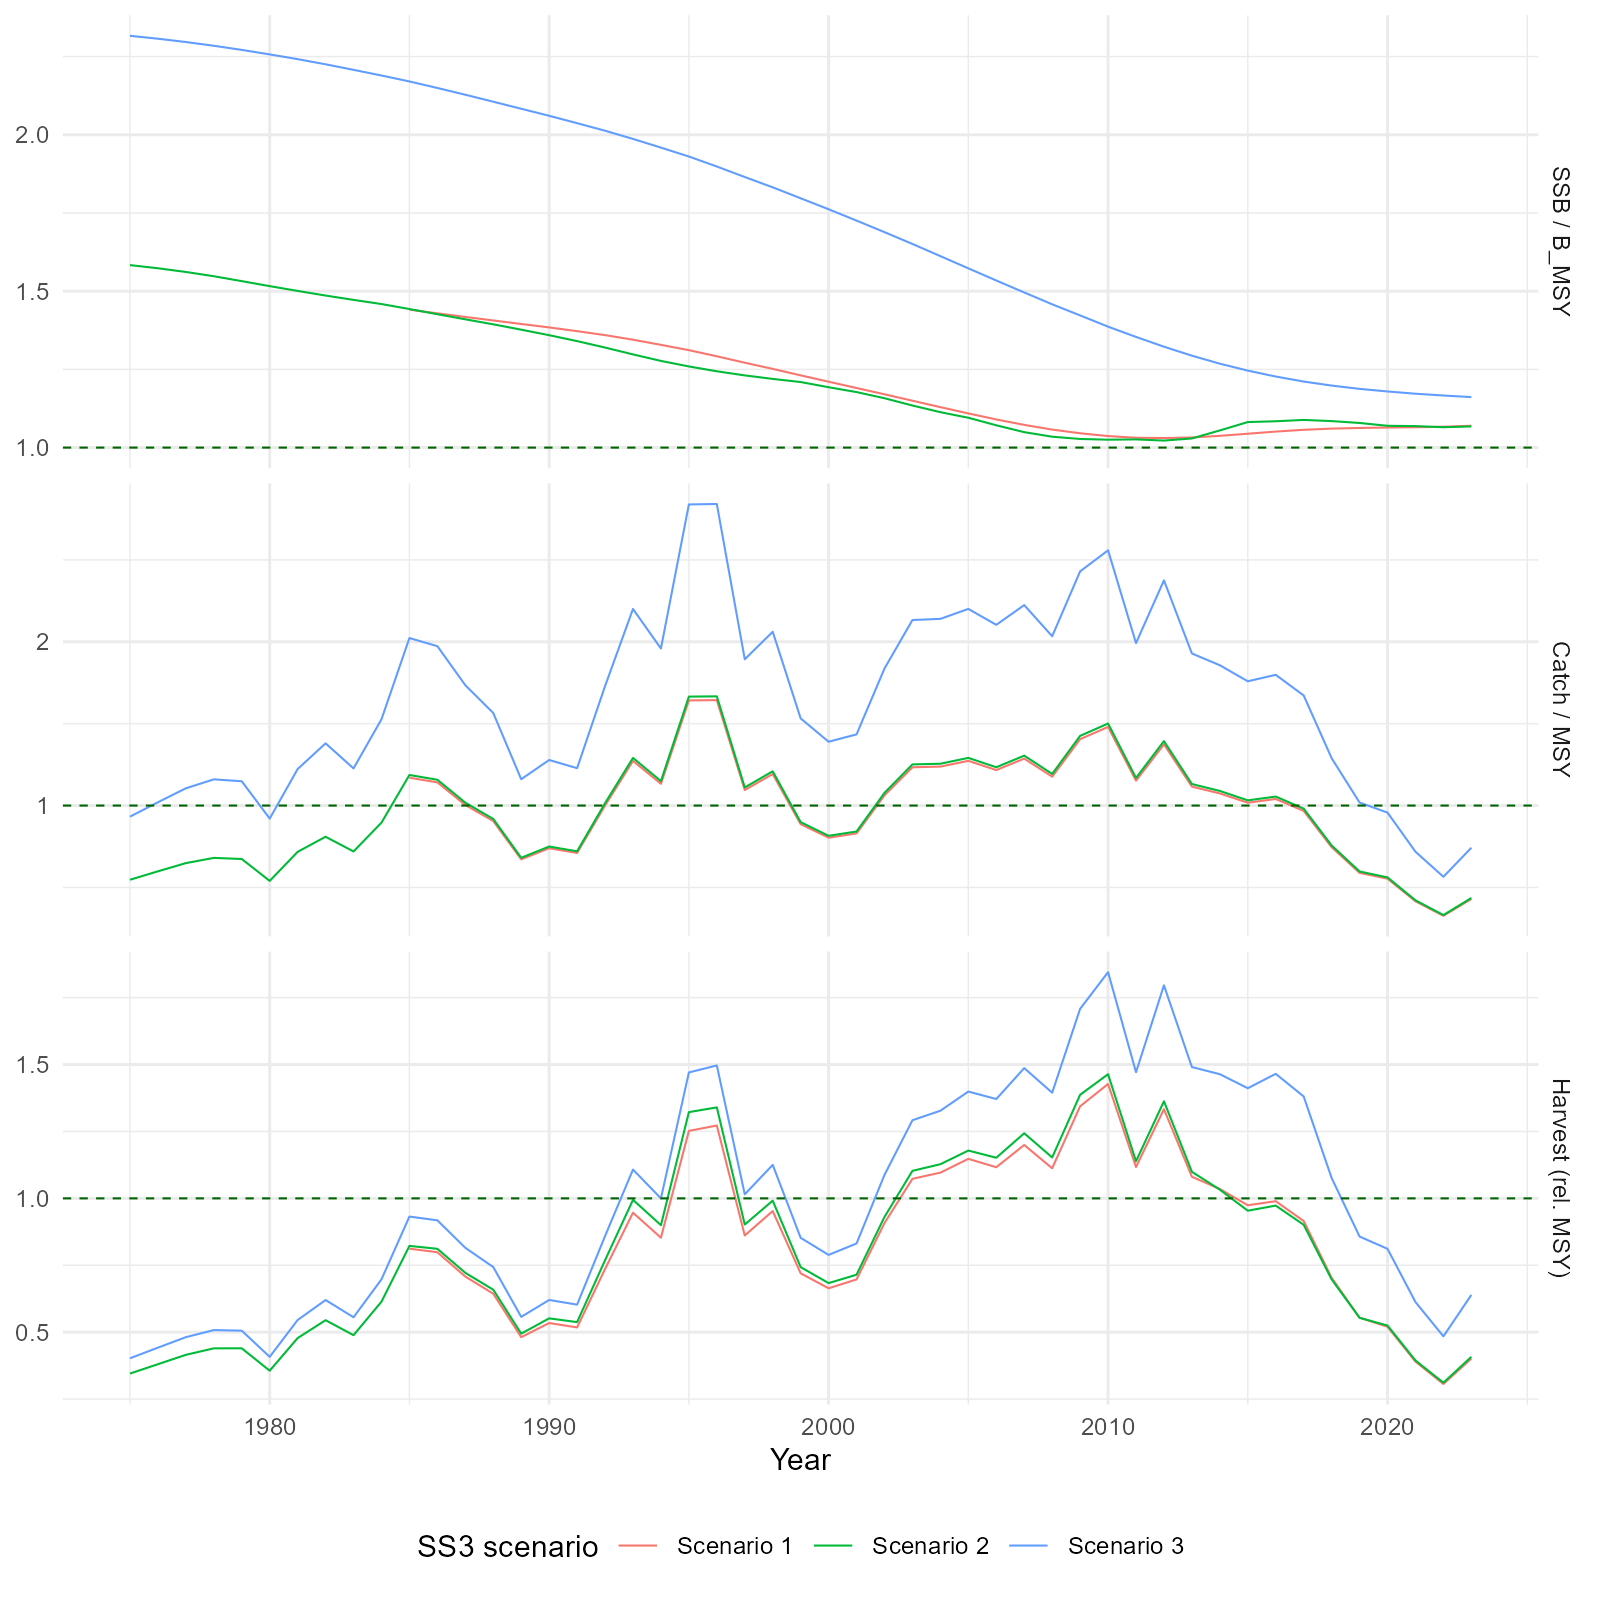
\includegraphics[width=0.92\linewidth]{figs/sma-fig-ts-1.png}
  \caption{MSY-scaled time series from the illustrative shortfin mako SS3 scenarios: spawning stock biomass, catch, and harvest intensity. Reproduced from the SS3 diagnostics prepared for SCRS/2026/074.}
  \label{fig:ts}
\end{figure}

\begin{figure}[H]
  \centering
  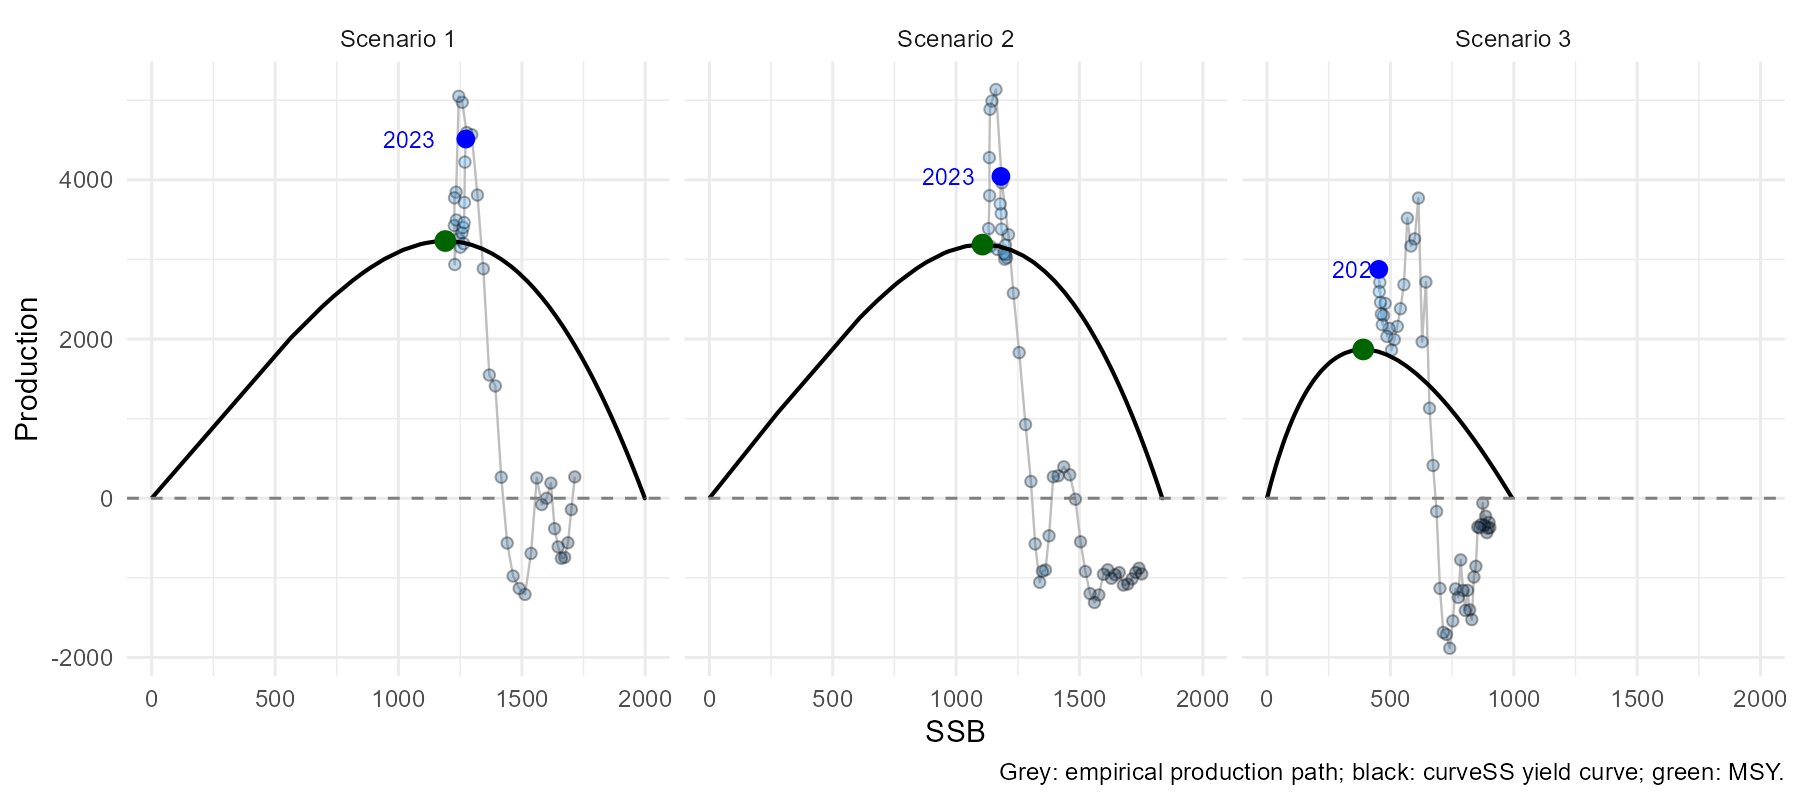
\includegraphics[width=0.92\linewidth]{figs/sma-fig-pe-phase-1.png}
  \caption{Equilibrium surplus-production curves with estimated production overlaid for the illustrative SS3 shortfin mako scenarios. Points and paths show annual estimated surplus production relative to spawning biomass.}
  \label{fig:pe-phase}
\end{figure}

These plots are internal diagnostics because they are derived from the fitted SS3 outputs and ask whether the implied dynamics behave as expected. They do not, by themselves, prove that the assessment is right or wrong. Instead, they identify where the internal accounting of biomass, production, removals, and reference points requires closer examination.

\subsection{External Diagnostics in the Case Study}
The main external diagnostic for shortfin mako is biological consistency: whether the fitted outputs and derived diagnostics agree with known maturity, selectivity, and age-structured response. The maturity and selectivity ogives differ strongly: fishing mortality acts heavily on ages below 50\% maturity, while the management state is mature female biomass. This creates a lag between changes in fishing mortality and changes in spawning biomass, weakens a simple instantaneous interpretation of surplus production on an SSB scale, and motivates the rebuilding-based diagnostics discussed below.

\begin{figure}[H]
  \centering
  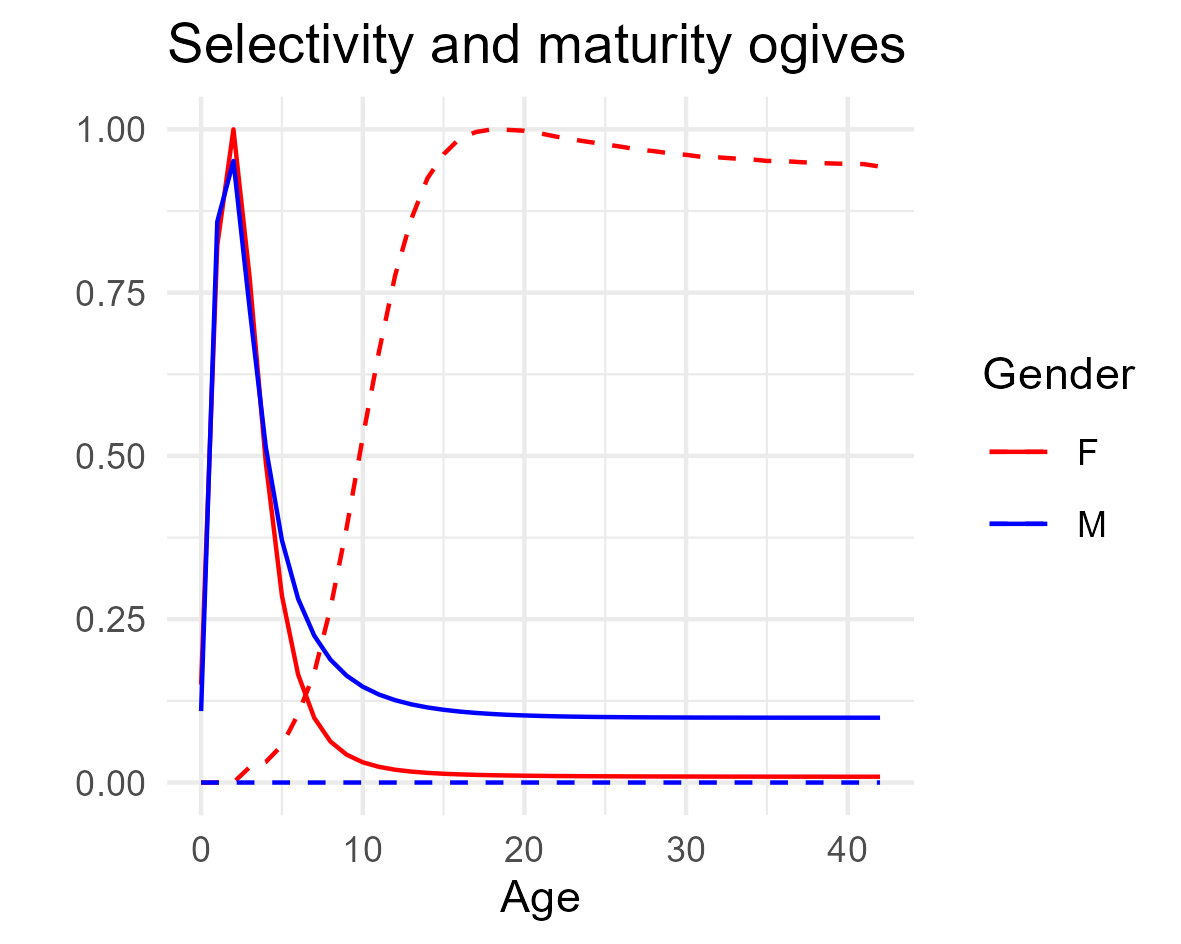
\includegraphics[width=0.88\linewidth]{figs/selmat.png}
  \caption{Comparison of selectivity and maturity-at-age in the illustrative shortfin mako SS3 scenarios. The mismatch is an external diagnostic because it is interpreted against life history and fishery selectivity, not only model fit.}
  \label{fig:selmat}
\end{figure}

This diagnostic changes the interpretation of the internal results. Negative or weak surplus production on an SSB scale may reflect a real productivity signal, but it may also reflect an inconsistent currency: the state is mature-female spawning biomass while removals are dominated by immature fish. External diagnostics therefore prevent over-interpreting a statistical residual as a direct biological process.

\subsection{Robustness Diagnostics in the Case Study}

Robustness diagnostics ask whether the advice-relevant conclusions remain stable when process error, non-stationarity, and alternative model structures are considered. SCRS/2026/074 examined residuals from the SS3-derived production functions over time, against biomass, as empirical distributions, and through autocorrelation. Structured residuals, regime-like shifts, biomass-dependent bias, or red-noise behaviour suggest that the fitted equilibrium production function is not fully summarising the stock dynamics.

\begin{figure}[H]
  \centering
  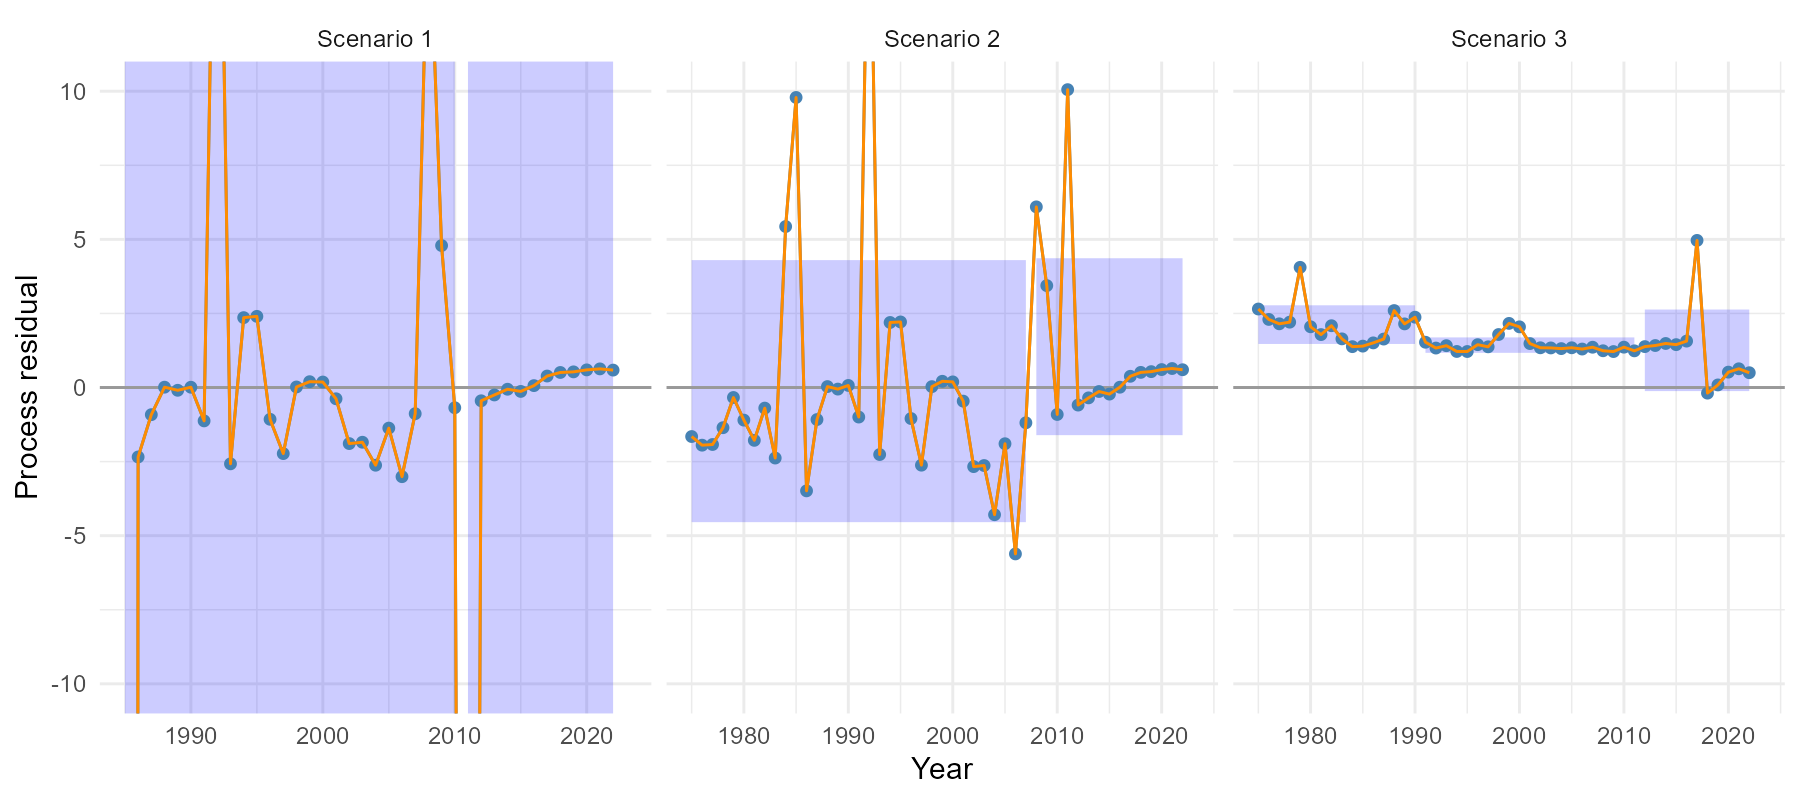
\includegraphics[width=0.92\linewidth]{figs/sma-fig-res-time-1.png}
  \caption{Process residuals over time for the illustrative shortfin mako SS3 scenarios. Shading identifies candidate regimes from a STARS-type filter \citep{rodionov2004sequential}.}
  \label{fig:res-time}
\end{figure}

\begin{figure}[H]
  \centering
  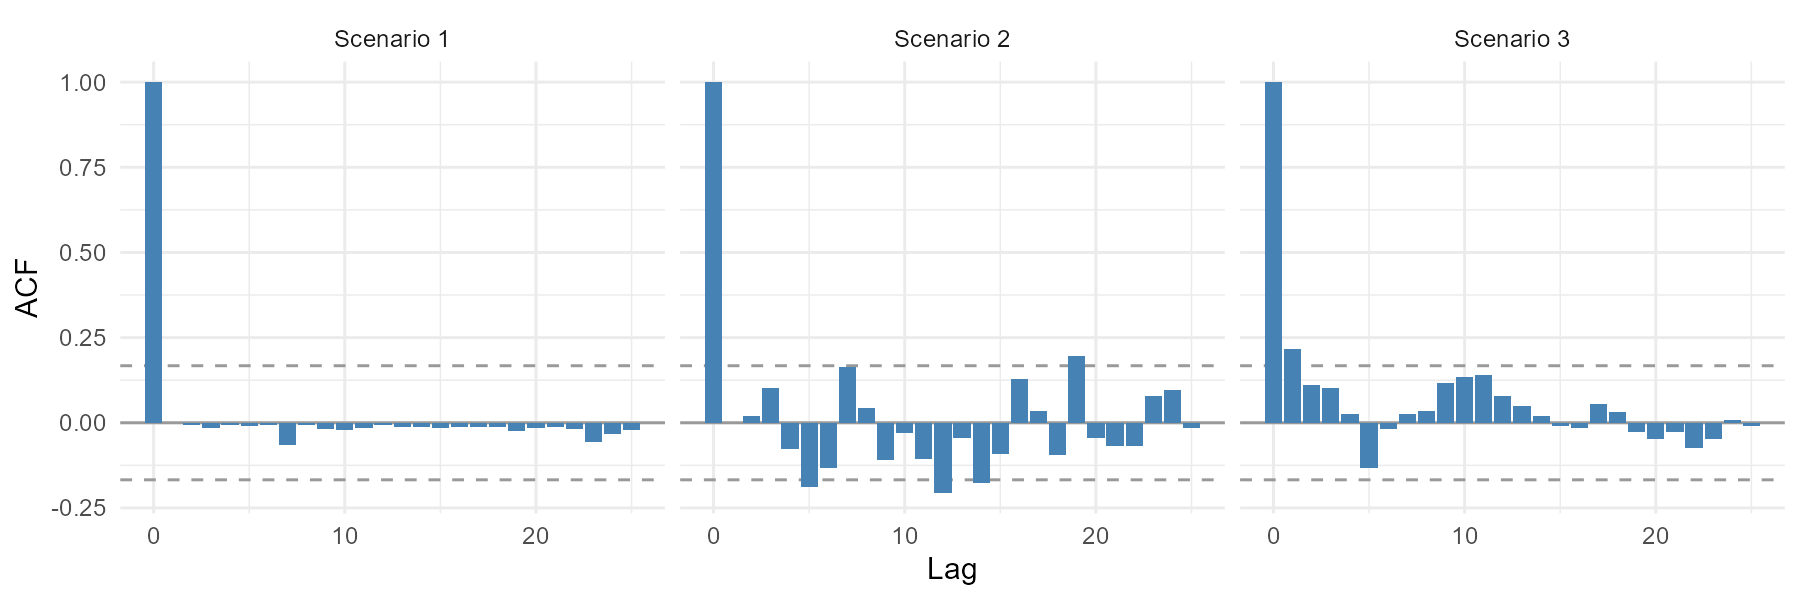
\includegraphics[width=0.92\linewidth]{figs/sma-fig-res-acf-1.png}
  \caption{Autocorrelation of process residuals for the illustrative SS3 shortfin mako scenarios. Autocorrelation in residuals is a robustness warning because it indicates that deviations are not behaving like independent process noise.}
  \label{fig:res-acf}
\end{figure}

The robustness message is that equilibrium reference points from a single SS3 configuration should be interpreted as conditional on the assumed dynamics. Where residuals are non-stationary or autocorrelated, and where state and removals are not expressed in a common biological currency, reference points and projections should be stress-tested through alternative scenarios, hindcasts, and management-strategy evaluation. In similar SCRS applications, residual diagnostics should be treated as a gating check before adopting equilibrium MSY reference points for advice.

\section{Lessons for SCRS Assessments}

The three diagnostic classes are complementary rather than hierarchical. For SCRS assessments using SS3 or similar integrated models, the accepted run and principal sensitivities should be accompanied by a compact checklist. The checklist is intended for the main paper or meeting report; the appendices can then hold the detailed plots, tables, and code-generated outputs.

\begin{enumerate}
  \item \textbf{Internal:} report convergence, maximum gradient, Hessian status, parameters near bounds, residual summaries by main data source, composition effective sample sizes, and information-content checks for advice-relevant quantities.
  \item \textbf{External:} report at least one maturity--selectivity or vulnerability plot, compare assessment trends with standardised survey perceptions, and state which spatial, environmental, or fishery signals are handled outside the assessment likelihood.
  \item \textbf{Robustness:} report retrospective patterns, at least one hindcast or prediction-skill check where feasible, key structural sensitivities, scenario or ensemble summaries for status and catch advice, tail probabilities for limits, and central tendencies for targets.
\end{enumerate}

This checklist also clarifies terminology. \textbf{Verification} asks whether the model and inputs are implemented correctly and reproducibly; for example, whether SS3 inputs, reported diagnostics, and residual plots can be regenerated from the archived files. \textbf{Validation} asks whether the model is adequate for its management use; for example, whether hindcasts have skill against withheld survey indices. \textbf{Uncertainty} describes the spread conditional on an accepted model, while \textbf{sensitivity} describes the spread across pre-specified model structures. Treating these as separate questions helps avoid confusing a well-fitted model with robust advice.

\section{Discussion}

Based on the shortfin mako SS3 case study, assessment diagnostics should be organised around the decision being supported. If the decision depends mainly on stock trend, then index fit, retrospective behaviour, and survey coherence may be most important. If the decision depends on MSY-based reference points, stock--recruitment information content, production-function behaviour, and sensitivity to steepness or productivity assumptions become central. If the decision depends on rebuilding, hindcasts, process-error diagnostics, and robustness of projections become more important.

\subsection{Rebuilding-based diagnostics for bycatch species}

For a non-retained bycatch species such as shortfin mako, MSY-based targets may be an inappropriate primary objective, particularly where fishing mortality is concentrated on juveniles and subadults while the management state is mature female spawning biomass \citep{winker2020age,Winker2025assessing}. In this setting, yield is not the management benefit being maximised, and the delay between reducing juvenile mortality and rebuilding the spawning component means that equilibrium $B_{\mathrm{MSY}}$ and $F_{\mathrm{MSY}}$ can be a poor summary of recovery potential.

Rebuilding-based quantities provide a more direct diagnostic frame:
\[
B_{\mathrm{rebuild}} = \min\{B_t : P(B_{t+T} \ge B_{\mathrm{target}} \mid F_{\mathrm{rebuild}}) \ge p^\ast\},
\]
where \(B_{\mathrm{rebuild}}\) is the lowest biomass from which the stock can reach an agreed target within horizon \(T\) under a stated fishing scenario, and \(p^\ast\) is an agreed probability. The complementary quantity \(T_{\mathrm{rebuild}}\) is the time required to reach that target from the current state \citep{kell2026rebuild}. For bycatch species, the target need not be \(B_{\mathrm{MSY}}\); it could be mature biomass, age structure, mature fraction, or another state-vector quantity linked to recovery and reproductive capacity \citep{griffiths2024including}.

The three diagnostic strands map naturally onto rebuilding. Internal diagnostics describe production-function behaviour and the fitted state vector. External diagnostics test whether maturity, selectivity, and age structure support the chosen rebuilding target. Robustness diagnostics report the distribution of \(T_{\mathrm{rebuild}}\), the probability of failing to rebuild within the agreed horizon, and sensitivity to alternative productivity or mortality assumptions. For example, an SCRS table could report \(P(B_T \ge B_{\mathrm{target}})\) over 20 or 30 years under a specified bycatch mortality scenario, alongside the median and upper quantiles of \(T_{\mathrm{rebuild}}\).

The shortfin mako example illustrates why internal diagnostics alone can be misleading. SS3 can provide a coherent fitted trajectory and reference points, yet the biological interpretation of production and process error depends on age structure and the currency of biomass and removals. External diagnostics identify that mismatch; robustness diagnostics then show whether management conclusions are sensitive to it.

For SCRS, a practical approach is to make the three diagnostic classes part of routine assessment documentation. The aim is not to require every possible diagnostic in every assessment cycle, but to make clear which questions have been answered, which are only partly addressed, and which remain open. This is particularly important when alternative model structures produce similar fits but different advice-relevant quantities. Appendices~\ref{app:internal}--\ref{app:robustness} provide stable wrapper structures for the three strands, with separate content files that can be populated as detailed diagnostics and code outputs become available; the main text should draw out decision-relevant examples rather than reproduce all diagnostic output.

\subsection{Role of the appendices}

The appendices are intended as reproducible diagnostic templates rather than fixed narrative sections. They provide the structure within which detailed plots, tables, and code outputs can be updated as generic functions are consolidated into R packages and case-study scripts are refined. This separation is useful for SCRS deadlines: the main paper can present the framework, rationale, and selected examples, while the appendices can expand as diagnostics are standardised and additional model runs become available.

In practice, reusable computation should live in packages or shared scripts, while the appendix Rmd files should remain thin case-study wrappers. Each appendix should record inputs, software versions, model runs, standard outputs, and the interpretation needed for review. This makes the appendices suitable both as technical documentation for a specific assessment and as templates for future SCRS case studies.

\section{Conclusions}

Internal, external, and robustness diagnostics answer different questions. Internal diagnostics test consistency with the fitted model and likelihood data. External diagnostics test biological and fishery consistency outside the likelihood. Robustness diagnostics test the stability of advice under pre-specified alternative structures and prediction-oriented checks.

The SS3 shortfin mako scenarios used for SCRS/2026/074 show how the three classes can be applied in practice without overloading the main paper. Production-function and residual diagnostics reveal structure that standard fits may not show; maturity and selectivity comparisons explain why some residual patterns are expected consequences of age structure; and robustness diagnostics indicate when reference points should be treated as conditional rather than definitive.

Routine SCRS reporting should present the three classes together, with clear separation of verification, validation, uncertainty, and sensitivity. A practical format is a concise main-body framework with selected examples, supported by reproducible appendices that hold detailed diagnostics and code-generated outputs. This would improve transparency, make structural uncertainty easier to communicate, and help ensure that assessment outputs are used in ways that are proportionate to their diagnostic support.

\section*{Acknowledgements}

We thank ICCAT and participants in the 2025 Shortfin Mako Shark Stock Assessment Meeting for making assessment materials available. The three-strand diagnostic framework draws on methods developed during an independent CIE review of the Bering Sea and Aleutian Islands yellowfin sole assessment. LK acknowledges financial support from the Spanish Surface Longline Fishing Sector producer organisations OPP-Burela, OPNAPA, OPROMAR, and ORPAGU under the 2026 collaboration agreement.

\appendix
\section{Internal Diagnostics and Reproducible Workflow}
\label{app:internal}

Internal diagnostics evaluate whether the fitted model is consistent with its likelihood,
parameterisation, and data inputs. This appendix provides a reproducible structure for
detailed case-study reporting. Generic computation should live in R packages; case-study
scripts should load inputs, call package functions, record software versions, and write
tables and figures into the content files below.

\subsection{Required R Packages}

\begin{table}

\caption{\label{tab:internal-libraries}Required R packages for internal diagnostics.}
\centering
\begin{tabular}[t]{llll}
\toprule
package & role & tier & installed\\
\midrule
knitr & Knit template; format LaTeX tables & core & 1.51\\
r4ss & Read SS3 output; summarise convergence and likelihood components & run\_code & 1.53.0\\
sstruth & curveSS, diagSS, ssU, ssLen, ssRunSummary, residual plots & run\_code & 0.0.0.9020\\
diags & CPUE diagnostic summaries via sstruth::ssU & run\_code & 2.2.1\\
ggplot2 & Likelihood, residual, and recruitment-deviation figures & run\_code & 4.0.3\\
\addlinespace
reshape2 & Data reshaping for diagnostic plots & run\_code & 1.4.5\\
ss3diags & SSrunstest and ssruns\_sig3; CPUE runs-test plots with 3-sigma limits & run\_code & 1.10.2\\
FLRebuild & Fallback curveSS if sstruth unavailable & planned & 0.1.0\\
ss3om & Fallback readFLSss3 via readTruth (optional) & planned & 0.5.3.9004\\
\bottomrule
\end{tabular}
\end{table}



\subsection{Inputs}

Record the accepted model run, principal sensitivities, software versions, and data
objects used to create this appendix.

\begin{table}

\caption{\label{tab:internal-inputs}Internal diagnostics inputs.}
\centering
\begin{tabular}[t]{ll}
\toprule
item & value\\
\midrule
Assessment ID & sma-ss3-2026\\
Model class & SS3\\
SS base directory & P:/rfmo/iccat/2026/shark/Analysis/ss3\\
Scenarios & Scenario\_1/Sc1\_Base, Scenario\_2/Scn02\_base, Scenario\_3/Sc3\_Base\\
Reference scenario & Scenario\_1/Sc1\_Base\\
\addlinespace
SS version & 3.30\\
R version & 4.4.2\\
r4ss & 1.53.0\\
ss3diags & 1.10.2\\
sstruth & 0.0.0.9020\\
\addlinespace
diags & 2.2.1\\
FLRebuild & 0.1.0\\
ss3om & 0.5.3.9004\\
Run code & TRUE\\
\bottomrule
\end{tabular}
\end{table}



\subsection{Standard Checks}

The minimum internal checklist should include:

\begin{itemize}
  \item convergence status, maximum gradient, Hessian status, and parameters near bounds;
  \item likelihood components and evidence for conflicts among data sources;
  \item residual diagnostics for indices and composition data;
  \item effective sample size diagnostics for composition data;
  \item likelihood profiles or equivalent information-content diagnostics for advice-relevant quantities;
  \item recruitment deviations and whether stock--recruitment assumptions are informed by data;
  \item process-error diagnostics: residuals versus time, biomass, ACF, and distributional properties (Appendix~\ref{app:internal}, process-error outputs).
\end{itemize}

% Internal diagnostic checks.

\begin{table}

\caption{\label{tab:internal-convergence}Convergence and Hessian summary by scenario.}
\centering
\begin{tabular}[t]{lrrrrrr}
\toprule
scenario & n\_params & total\_ll & max\_grad & log\_det\_hessian & n\_iterations & n\_warnings\\
\midrule
Scenario-1 & 92 & 515.254 & 5.67e-05 & 134.9 & 801 & 7\\
Scenario-2 & 100 & 485.295 & 1.06e-05 & 160.9 & 863 & 6\\
Scenario-3 & 109 & 1164.320 & 9.18e-05 & 173.2 & 1061 & 6\\
\bottomrule
\end{tabular}
\end{table}

\begin{table}

\caption{\label{tab:internal-ll-components}Likelihood components for the reference scenario.}
\centering
\begin{tabular}[t]{llrr}
\toprule
  & component & log\_likelihood & lambda\\
\midrule
5 & Length\_comp & 613.162 & NA\\
4 & Survey & -88.782 & NA\\
6 & Recruitment & -10.025 & 1\\
9 & Parm\_priors & 0.772 & 1\\
8 & Forecast\_Recruitment & 0.111 & 1\\
\addlinespace
10 & Parm\_softbounds & 0.015 & NA\\
2 & Catch & 0.000 & NA\\
3 & Equil\_catch & 0.000 & NA\\
7 & InitEQ\_Regime & 0.000 & 1\\
11 & Parm\_devs & 0.000 & 1\\
\addlinespace
12 & Crash\_Pen & 0.000 & 1\\
\bottomrule
\end{tabular}
\end{table}

% No estimated parameters within 2 percent of bounds (reference scenario).

\begin{table}

\caption{\label{tab:internal-advice-pars}Advice-relevant parameters and asymptotic standard errors (reference scenario).}
\centering
\begin{tabular}[t]{llrrrrlr}
\toprule
  & Label & Value & Phase & Min & Max & Status & se\\
\midrule
SR\_autocorr & SR\_autocorr & 0.000000 & -4 & -5.00 & 5.00 & NA & NA\\
SR\_LN(R0) & SR\_LN(R0) & 5.528090 & 1 & 2.30 & 13.82 & OK & 0.126584\\
SR\_regime & SR\_regime & 0.000000 & -4 & -5.00 & 5.00 & NA & NA\\
SR\_sigmaR & SR\_sigmaR & 0.283103 & -4 & 0.20 & 1.90 & NA & NA\\
SR\_surv\_Beta & SR\_surv\_Beta & 3.000000 & -4 & 0.01 & 10.00 & NA & NA\\
\addlinespace
SR\_surv\_zfrac & SR\_surv\_zfrac & 0.372000 & -4 & 0.01 & 1.00 & NA & NA\\
\bottomrule
\end{tabular}
\end{table}

\begin{table}

\caption{\label{tab:internal-comp-ess}Length-composition effective sample size summary by fleet (sstruth::ssLen).}
\centering
\begin{tabular}[t]{lrrrlrrrrrrlrlllllrrrl}
\toprule
  & Data\_type & Fleet & Recommend\_var\_adj & \# & N & Npos & min\_Nsamp & max\_Nsamp & mean\_Nsamp\_in & mean\_Nsamp\_adj & mean\_Nsamp\_DM & err\_method & err\_index & par1 & val1 & par2 & val2 & mean\_effN & HarMean & Curr\_Var\_Adj & Fleet\_name\\
\midrule
3618 & 4 & 1 & 1.595300 & \# & 22 & 22 & 4.10135 & 26.88660 & 22.63640 & 10.31550 & NA & 0 & NA & multinomial & NA & NA & NA & 73.2504 & 36.1118 & 0.455705 & F01\_EU\_SPN\\
3619 & 4 & 2 & 3.348320 & \# & 13 & 13 & 5.75133 & 9.58555 & 11.07690 & 7.07856 & NA & 0 & NA & multinomial & NA & NA & NA & 40.8450 & 37.0890 & 0.639037 & F02\_EU\_POR\\
3620 & 4 & 3 & 4.379130 & \# & 15 & 15 & 7.08631 & 18.22190 & 10.53330 & 10.66320 & NA & 0 & NA & multinomial & NA & NA & NA & 49.4968 & 46.1268 & 1.012330 & F03\_JPN\\
3621 & 4 & 4 & 1.711010 & \# & 4 & 4 & 2.57489 & 6.11536 & 11.50000 & 3.70140 & NA & 0 & NA & multinomial & NA & NA & NA & 22.9236 & 19.6766 & 0.321861 & F04\_CTP\\
3622 & 4 & 5 & 6.092490 & \# & 24 & 24 & 10.60390 & 37.87100 & 13.95830 & 21.14460 & NA & 0 & NA & multinomial & NA & NA & NA & 103.6380 & 85.0410 & 1.514840 & F05\_USA\\
\addlinespace
3623 & 4 & 6 & 3.428940 & \# & 14 & 14 & 3.09308 & 6.62804 & 10.28570 & 4.54494 & NA & 0 & NA & multinomial & NA & NA & NA & 50.2229 & 35.2691 & 0.441869 & F06\_CAN\\
3624 & 4 & 7 & 0.983769 & \# & 6 & 6 & 6.03750 & 34.21250 & 23.33330 & 23.47920 & NA & 0 & NA & multinomial & NA & NA & NA & 28.7302 & 22.9546 & 1.006250 & F07\_MOR\\
3625 & 4 & 8 & 5.842330 & \# & 22 & 22 & 21.53180 & 36.91160 & 9.18182 & 28.24300 & NA & 0 & NA & multinomial & NA & NA & NA & 61.8055 & 53.6432 & 3.075970 & F08\_MEX\\
3626 & 4 & 9 & 4.599110 & \# & 2 & 2 & 41.42290 & 55.23050 & 10.50000 & 48.32670 & NA & 0 & NA & multinomial & NA & NA & NA & 48.3984 & 48.2906 & 4.602540 & F09\_VEN\\
\bottomrule
\end{tabular}
\end{table}

\begin{table}

\caption{\label{tab:internal-ssu-summary}CPUE residual summary by fleet (sstruth::diagSS / ssU).}
\centering
\begin{tabular}[t]{lrrrr}
\toprule
name & n & mean\_abs\_residual & max\_abs\_std & runs\_p\\
\midrule
CPUE\_CTP & 11 & 0.59710 & NA & NA\\
CPUE\_EU\_POR & 25 & 0.25710 & NA & NA\\
CPUE\_EU\_SPN & 34 & 0.21250 & NA & NA\\
CPUE\_JPN\_1 & 14 & 0.13170 & NA & NA\\
CPUE\_JPN\_2 & 15 & 0.23190 & NA & NA\\
\addlinespace
CPUE\_MOR\_1 & 10 & 0.16010 & NA & NA\\
CPUE\_MOR\_2 & 2 & 0.08311 & NA & NA\\
CPUE\_USA & 32 & 0.28830 & NA & NA\\
CPUE\_USAlogbook & 30 & 0.19000 & NA & NA\\
\bottomrule
\end{tabular}
\end{table}

% SS3 run notes from sstruth::ssRunSummary:
% warning_excerpt: Note 1 Information: Max data length bin: 320  < max pop len bins: 380; so will accumulate larger pop len bins
% warning_excerpt: Warning 1 Adjustment: basis for HCR anchor was not set; setting to 2 to match default before 3.30.24
% warning_excerpt: Warning 2 : parm min for Lmin: 5 should not be less than population min length bin 35
% warning_excerpt: Note 2 Suggestion: Are you sure you want so few early recrdevs? Better to include in range of main recdevs 5
% warning_excerpt: Warning 3 : Setting in starter does not request all priors, and 40 parameters have priors and are not estimated, so their prior not included in obj_fun.
% warning_excerpt: Note 3 Information: A revised protocol for the Fcast_yr specification is available and recommended.
% warning_excerpt:  3 warnings  and 3 notes 

\begin{table}

\caption{\label{tab:internal-index-tuning}Index variance tuning and RMSE by CPUE fleet.}
\centering
\begin{tabular}[t]{lllllllll}
\toprule
  & Fleet & N & Npos & RMSE & Input+VarAdj+extra & VarAdj & New\_VarAdj & fleetname\\
\midrule
3455 & 12 & 34 & 34 & 0.315849 & 0.252706 & 0.132 & 0.327143 & CPUE\_EU\_SPN\\
3456 & 13 & 25 & 25 & 0.394276 & 0.43312 & 0 & -0.0388442 & CPUE\_EU\_POR\\
3457 & 14 & 14 & 14 & 0.175758 & 0.214643 & 0.163 & 0.287115 & CPUE\_JPN\_1\\
3458 & 15 & 15 & 15 & 0.286788 & 0.3668 & 0 & -0.0800123 & CPUE\_JPN\_2\\
3459 & 16 & 11 & 11 & 0.722256 & 0.326909 & 0.165 & 0.725347 & CPUE\_CTP\\
\addlinespace
3460 & 17 & 32 & 32 & 0.343423 & 0.273438 & 0.022 & 0.113985 & CPUE\_USA\\
3461 & 18 & 10 & 10 & 0.212431 & 0.2545 & 0.129 & 0.215931 & CPUE\_MOR\_1\\
3462 & 19 & 2 & 2 & 0.0831072 & 0.2005 & 0.01 & -0.0973928 & CPUE\_MOR\_2\\
3463 & 20 & 30 & 30 & 0.247158 & 0.210087 & 0.12 & 0.277072 & CPUE\_USAlogbook\\
\bottomrule
\end{tabular}
\end{table}

\begin{table}

\caption{\label{tab:internal-runs-test}CPUE residual runs-test summary by fleet (ss3diags::SSrunstest).}
\centering
\begin{tabular}[t]{lrlrrl}
\toprule
Index & runs.p & test & sigma3.lo & sigma3.hi & type\\
\midrule
CPUE\_EU\_SPN & 0.249 & Passed & -0.4816 & 0.4816 & cpue\\
CPUE\_EU\_POR & 0.272 & Passed & -0.7635 & 0.7635 & cpue\\
CPUE\_JPN\_1 & 0.013 & Failed & -0.3828 & 0.3828 & cpue\\
CPUE\_JPN\_2 & 0.092 & Passed & -0.8176 & 0.8176 & cpue\\
CPUE\_CTP & 0.475 & Passed & -2.0140 & 2.0140 & cpue\\
\addlinespace
CPUE\_USA & 0.145 & Passed & -0.6970 & 0.6970 & cpue\\
CPUE\_MOR\_1 & 0.103 & Passed & -0.5004 & 0.5004 & cpue\\
CPUE\_MOR\_2 & NA & Excluded & NA & NA & cpue\\
CPUE\_USAlogbook & 0.000 & Failed & -0.2873 & 0.2873 & cpue\\
\bottomrule
\end{tabular}
\end{table}

\begin{table}

\caption{\label{tab:internal-runs-qic}CPUE residual individual-chart runs tests by fleet (crossings and longest-run criteria).}
\centering
\begin{tabular}[t]{llrrrrlll}
\toprule
scenario & name & n.crossings & n.crossings.min & longest.run & longest.run.max & crossings & runs & Pass\\
\midrule
Scenario 1 & CPUE\_CTP & 5 & 2 & 4 & 6 & TRUE & TRUE & TRUE\\
Scenario 1 & CPUE\_EU\_POR & 11 & 6 & 3 & 7 & TRUE & TRUE & TRUE\\
Scenario 1 & CPUE\_EU\_SPN & 15 & 8 & 6 & 8 & TRUE & TRUE & TRUE\\
Scenario 1 & CPUE\_JPN\_1 & 3 & 3 & 5 & 6 & FALSE & TRUE & FALSE\\
Scenario 1 & CPUE\_JPN\_2 & 5 & 3 & 6 & 6 & TRUE & FALSE & FALSE\\
\addlinespace
Scenario 1 & CPUE\_MOR\_1 & 3 & 2 & 3 & 6 & TRUE & TRUE & TRUE\\
Scenario 1 & CPUE\_MOR\_2 & 1 & 0 & 1 & 3 & TRUE & TRUE & TRUE\\
Scenario 1 & CPUE\_USA & 13 & 7 & 6 & 7 & TRUE & TRUE & TRUE\\
Scenario 1 & CPUE\_USAlogbook & 3 & 7 & 12 & 7 & FALSE & FALSE & FALSE\\
\bottomrule
\end{tabular}
\end{table}

\begin{table}

\caption{\label{tab:internal-rec-sigma}Recruitment deviation summary statistics from SS3 report.}
\centering
\begin{tabular}[t]{lrrrrrrrrl}
\toprule
period & N\_devs & SD\_of\_devs & Var\_of\_devs & mean\_SE & mean\_SEsquared & sqrt\_sum\_of\_components & SD\_of\_devs\_over\_sigma\_R & sqrt\_sum\_over\_sigma\_R & alternative\_sigma\_R\\
\midrule
Main & 31 & 0.1805979 & 0.0326156 & 0.1971533 & 0.0391536 & 0.2678978 & 0.6379228 & 0.9462909 & 0.26789779814548\\
Early+Main & 36 & 0.1758351 & 0.0309180 & 0.2051770 & 0.0427470 & 0.2714129 & 0.6210994 & 0.9587074 & 0.271412929542226\\
Early+Main+Late & 39 & 0.1705995 & 0.0291042 & 0.2090008 & 0.0444819 & 0.2712676 & 0.6026058 & 0.9581939 & 0.271267571442131\\
\bottomrule
\end{tabular}
\end{table}

\begin{table}

\caption{\label{tab:internal-rec-rmse}Recruitment-deviation RMSE and Durbin-Watson diagnostics.}
\centering
\begin{tabular}[t]{lrrrrrr}
\toprule
ERA & N & RMSE & RMSE\textasciicircum{}2/sigmaR\textasciicircum{}2 & mean\_BiasAdj & est\_rho & Durbin-Watson\\
\midrule
main & 31 & 0.177661 & 0.393818 & 0.376244 & 0.602694 & 0.778993\\
early & 5 & 0.155099 & 0.300142 & 0.229362 & NA & NA\\
\bottomrule
\end{tabular}
\end{table}

\begin{table}

\caption{\label{tab:internal-profile-manifest}Likelihood-profile SS3 run manifest (M $\times$ SR\_surv\_Beta grid).}
\centering
\begin{tabular}[t]{rrlrl}
\toprule
M & beta & dir & total\_ll & ok\\
\midrule
0.500 & 0.5 & C:/active/scrs-papers/ss-ll/data/ICCAT\_2017\_Model\_Run\_3\_SSv330.23.02/00\_Model\_run\_files/0.5/0.5 & 83.2768 & TRUE\\
0.500 & 1.0 & C:/active/scrs-papers/ss-ll/data/ICCAT\_2017\_Model\_Run\_3\_SSv330.23.02/00\_Model\_run\_files/0.5/1 & 82.8158 & TRUE\\
0.500 & 1.5 & C:/active/scrs-papers/ss-ll/data/ICCAT\_2017\_Model\_Run\_3\_SSv330.23.02/00\_Model\_run\_files/0.5/1.5 & 82.4124 & TRUE\\
0.625 & 0.5 & C:/active/scrs-papers/ss-ll/data/ICCAT\_2017\_Model\_Run\_3\_SSv330.23.02/00\_Model\_run\_files/0.625/0.5 & 80.4027 & TRUE\\
0.625 & 1.0 & C:/active/scrs-papers/ss-ll/data/ICCAT\_2017\_Model\_Run\_3\_SSv330.23.02/00\_Model\_run\_files/0.625/1 & 79.9028 & TRUE\\
\addlinespace
0.625 & 1.5 & C:/active/scrs-papers/ss-ll/data/ICCAT\_2017\_Model\_Run\_3\_SSv330.23.02/00\_Model\_run\_files/0.625/1.5 & 79.4653 & TRUE\\
0.750 & 0.5 & C:/active/scrs-papers/ss-ll/data/ICCAT\_2017\_Model\_Run\_3\_SSv330.23.02/00\_Model\_run\_files/0.75/0.5 & 79.0489 & TRUE\\
0.750 & 1.0 & C:/active/scrs-papers/ss-ll/data/ICCAT\_2017\_Model\_Run\_3\_SSv330.23.02/00\_Model\_run\_files/0.75/1 & 78.5454 & TRUE\\
0.750 & 1.5 & C:/active/scrs-papers/ss-ll/data/ICCAT\_2017\_Model\_Run\_3\_SSv330.23.02/00\_Model\_run\_files/0.75/1.5 & 78.1602 & TRUE\\
0.875 & 0.5 & C:/active/scrs-papers/ss-ll/data/ICCAT\_2017\_Model\_Run\_3\_SSv330.23.02/00\_Model\_run\_files/0.875/0.5 & 78.5405 & TRUE\\
\addlinespace
0.875 & 1.0 & C:/active/scrs-papers/ss-ll/data/ICCAT\_2017\_Model\_Run\_3\_SSv330.23.02/00\_Model\_run\_files/0.875/1 & 78.1173 & TRUE\\
0.875 & 1.5 & C:/active/scrs-papers/ss-ll/data/ICCAT\_2017\_Model\_Run\_3\_SSv330.23.02/00\_Model\_run\_files/0.875/1.5 & 77.6292 & TRUE\\
1.000 & 0.5 & C:/active/scrs-papers/ss-ll/data/ICCAT\_2017\_Model\_Run\_3\_SSv330.23.02/00\_Model\_run\_files/1/0.5 & 78.5944 & TRUE\\
1.000 & 1.0 & C:/active/scrs-papers/ss-ll/data/ICCAT\_2017\_Model\_Run\_3\_SSv330.23.02/00\_Model\_run\_files/1/1 & 78.0832 & TRUE\\
1.000 & 1.5 & C:/active/scrs-papers/ss-ll/data/ICCAT\_2017\_Model\_Run\_3\_SSv330.23.02/00\_Model\_run\_files/1/1.5 & 77.6315 & TRUE\\
\addlinespace
1.125 & 0.5 & C:/active/scrs-papers/ss-ll/data/ICCAT\_2017\_Model\_Run\_3\_SSv330.23.02/00\_Model\_run\_files/1.125/0.5 & 78.8160 & TRUE\\
1.125 & 1.0 & C:/active/scrs-papers/ss-ll/data/ICCAT\_2017\_Model\_Run\_3\_SSv330.23.02/00\_Model\_run\_files/1.125/1 & 78.3617 & TRUE\\
1.125 & 1.5 & C:/active/scrs-papers/ss-ll/data/ICCAT\_2017\_Model\_Run\_3\_SSv330.23.02/00\_Model\_run\_files/1.125/1.5 & 77.9736 & TRUE\\
1.250 & 0.5 & C:/active/scrs-papers/ss-ll/data/ICCAT\_2017\_Model\_Run\_3\_SSv330.23.02/00\_Model\_run\_files/1.25/0.5 & 79.2123 & TRUE\\
1.250 & 1.0 & C:/active/scrs-papers/ss-ll/data/ICCAT\_2017\_Model\_Run\_3\_SSv330.23.02/00\_Model\_run\_files/1.25/1 & 78.8435 & TRUE\\
\addlinespace
1.250 & 1.5 & C:/active/scrs-papers/ss-ll/data/ICCAT\_2017\_Model\_Run\_3\_SSv330.23.02/00\_Model\_run\_files/1.25/1.5 & 78.5343 & TRUE\\
1.375 & 0.5 & C:/active/scrs-papers/ss-ll/data/ICCAT\_2017\_Model\_Run\_3\_SSv330.23.02/00\_Model\_run\_files/1.375/0.5 & 79.7198 & TRUE\\
1.375 & 1.0 & C:/active/scrs-papers/ss-ll/data/ICCAT\_2017\_Model\_Run\_3\_SSv330.23.02/00\_Model\_run\_files/1.375/1 & 79.4526 & TRUE\\
1.375 & 1.5 & C:/active/scrs-papers/ss-ll/data/ICCAT\_2017\_Model\_Run\_3\_SSv330.23.02/00\_Model\_run\_files/1.375/1.5 & 79.2327 & TRUE\\
1.500 & 0.5 & C:/active/scrs-papers/ss-ll/data/ICCAT\_2017\_Model\_Run\_3\_SSv330.23.02/00\_Model\_run\_files/1.5/0.5 & 80.7181 & TRUE\\
\addlinespace
1.500 & 1.0 & C:/active/scrs-papers/ss-ll/data/ICCAT\_2017\_Model\_Run\_3\_SSv330.23.02/00\_Model\_run\_files/1.5/1 & 80.6296 & TRUE\\
1.500 & 1.5 & C:/active/scrs-papers/ss-ll/data/ICCAT\_2017\_Model\_Run\_3\_SSv330.23.02/00\_Model\_run\_files/1.5/1.5 & 80.5685 & TRUE\\
\bottomrule
\end{tabular}
\end{table}



\subsection{Process Error and Stock--Recruitment Diagnostics}

Process-error diagnostics follow the four-panel structure described in Section~2.1 of the main text: temporal patterns (including regime-shift filters such as STARS), biomass-dependent bias, autocorrelation structure, and distributional properties. Where stock--recruitment relationships are fitted externally to assessment outputs, report whether uncertainty in SSB and recruitment was propagated; internal state-space formulations (e.g.\ SAM) should be distinguished from post-hoc fits to SS3 point estimates.

% Process-error diagnostic outputs (curveSS).

\begin{figure}[H]
  \centering
  \includegraphics[width=0.95\linewidth]{appendices/figs/internal/production-functions-scenarios.png}
  \caption{Production functions by SS3 scenario (curveSS; historical SSB--yield trajectory; Kobe quadrants, MSY, 40\% $B_\mathrm{max}$ path).}
  \label{fig:internal-production-functions-scenarios}
\end{figure}

\begin{figure}[H]
  \centering
  \includegraphics[width=0.95\linewidth]{appendices/figs/internal/kobe-phase-scenarios.png}
  \caption{Kobe phase plot by SS3 scenario (curveSS).}
  \label{fig:internal-kobe-phase-scenarios}
\end{figure}

\begin{figure}[H]
  \centering
  \includegraphics[width=0.92\linewidth]{appendices/figs/internal/pe-four-panel.png}
  \caption{Four-panel process-error diagnostics (curveSS).}
  \label{fig:internal-pe-four-panel}
\end{figure}


\subsection{Diagnostic Output}

Tables, figures, and code-generated summaries can be added to the file below as they
become available.

% Internal diagnostic figures and tables.

\begin{figure}[H]
  \centering
  \includegraphics[width=0.92\linewidth]{appendices/figs/internal/ss3-ts.png}
  \caption{SS3 scenario time series relative to MSY reference points (from curveSS).}
  \label{fig:internal-ss3-ts}
\end{figure}

\begin{figure}[H]
  \centering
  \includegraphics[width=0.92\linewidth]{appendices/figs/internal/ss3-pe-phase.png}
  \caption{Empirical production and curveSS yield curve versus spawning stock biomass.}
  \label{fig:internal-ss3-pe-phase}
\end{figure}

\begin{figure}[H]
  \centering
  \includegraphics[width=0.92\linewidth]{appendices/figs/internal/cpue-fit.png}
  \caption{Observed and expected CPUE indices (sstruth::diagSS).}
  \label{fig:internal-cpue-fit}
\end{figure}

\begin{figure}[H]
  \centering
  \includegraphics[width=0.92\linewidth]{appendices/figs/internal/cpue-residuals.png}
  \caption{CPUE residuals by fleet (sstruth::plotResiduals).}
  \label{fig:internal-cpue-residuals}
\end{figure}

\begin{figure}[H]
  \centering
  \includegraphics[width=0.92\linewidth]{appendices/figs/internal/cpue-std-residuals.png}
  \caption{Standardised CPUE residuals (sstruth::plotStdResiduals).}
  \label{fig:internal-cpue-std-residuals}
\end{figure}

\begin{figure}[H]
  \centering
  \includegraphics[width=0.95\linewidth]{appendices/figs/internal/cpue-runs-test.png}
  \caption{CPUE residual runs tests by fleet (individual-chart criteria; cf. figures.Rmd jara-runs).}
  \label{fig:internal-cpue-runs}
\end{figure}

\begin{figure}[H]
  \centering
  \includegraphics[width=0.95\linewidth]{appendices/figs/internal/cpue-runs-sig3.png}
  \caption{CPUE residual runs tests with 3-sigma limits (ss3diags::SSrunstest).}
  \label{fig:internal-cpue-runs-sig3}
\end{figure}

\begin{figure}[H]
  \centering
  \includegraphics[width=0.88\linewidth]{appendices/figs/internal/ll-components.png}
  \caption{Likelihood components for the reference scenario.}
  \label{fig:internal-ll-components}
\end{figure}

\begin{figure}[H]
  \centering
  \includegraphics[width=0.92\linewidth]{appendices/figs/internal/rec-devs.png}
  \caption{Recruitment deviations for the reference scenario.}
  \label{fig:internal-rec-devs}
\end{figure}

\begin{figure}[H]
  \centering
  \includegraphics[width=0.92\linewidth]{appendices/figs/internal/len-comp-residual-f1.png}
  \caption{Length-composition residuals, fleet 1 (sstruth::ssLen when available).}
  \label{fig:internal-len-comp-residual}
\end{figure}

\begin{figure}[H]
  \centering
  \includegraphics[width=0.88\linewidth]{appendices/figs/internal/ll-profile-total.png}
  \caption{Total log-likelihood profile over M and SR\_surv\_Beta fixed parameters.}
  \label{fig:internal-ll-profile-total}
\end{figure}

\begin{figure}[H]
  \centering
  \includegraphics[width=0.95\linewidth]{appendices/figs/internal/ll-profile-components.png}
  \caption{Likelihood-profile components by data source (M $\times$ SR\_surv\_Beta grid).}
  \label{fig:internal-ll-profile-components}
\end{figure}

\begin{figure}[H]
  \centering
  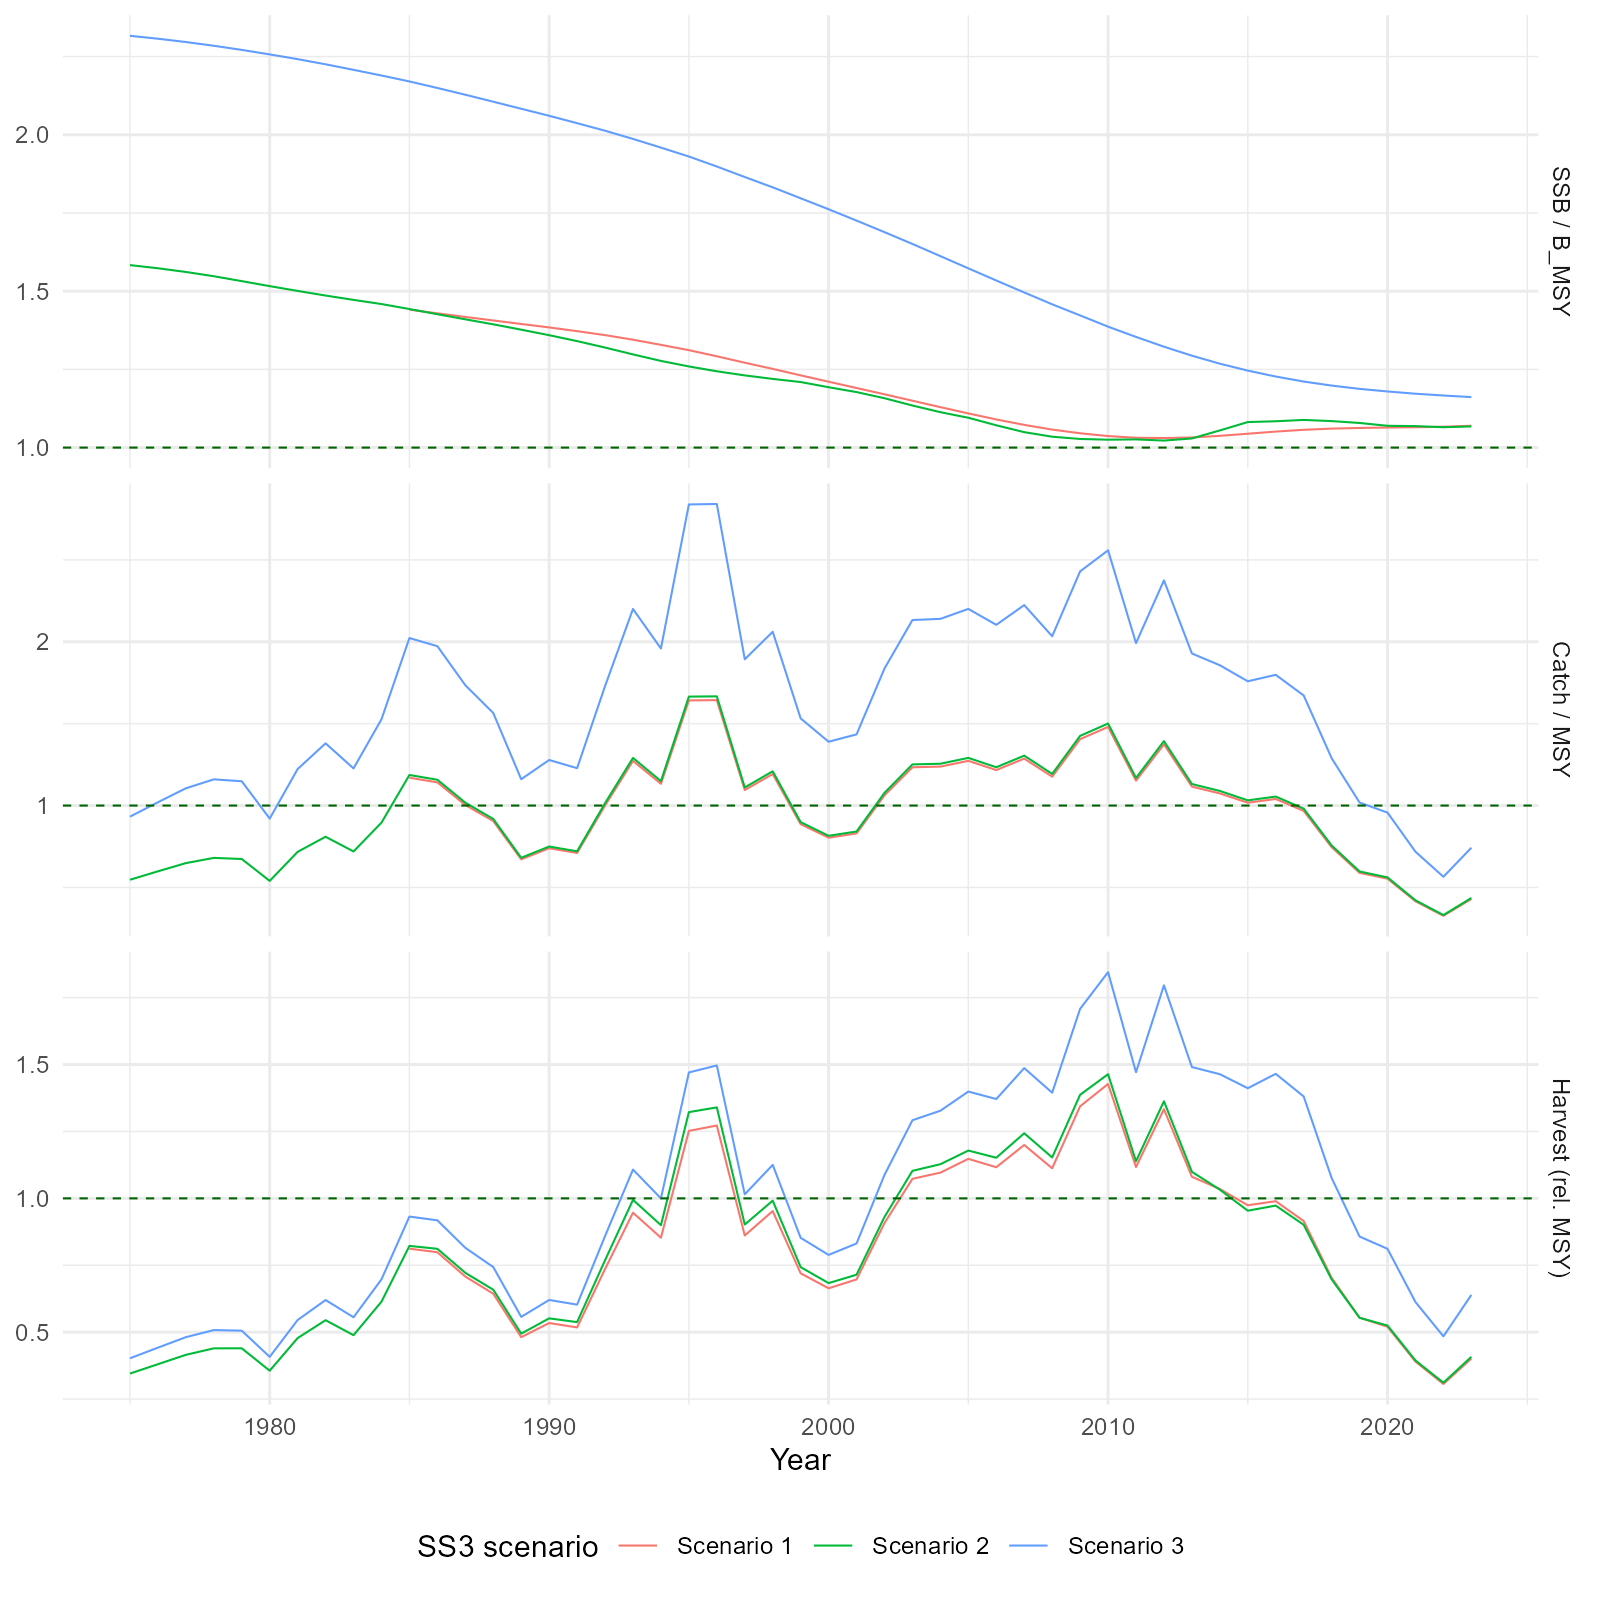
\includegraphics[width=0.92\linewidth]{figs/sma-fig-ts-1.png}
  \caption{sma fig ts 1}
  \label{fig:internal-sma-fig-ts-1}
\end{figure}

\begin{figure}[H]
  \centering
  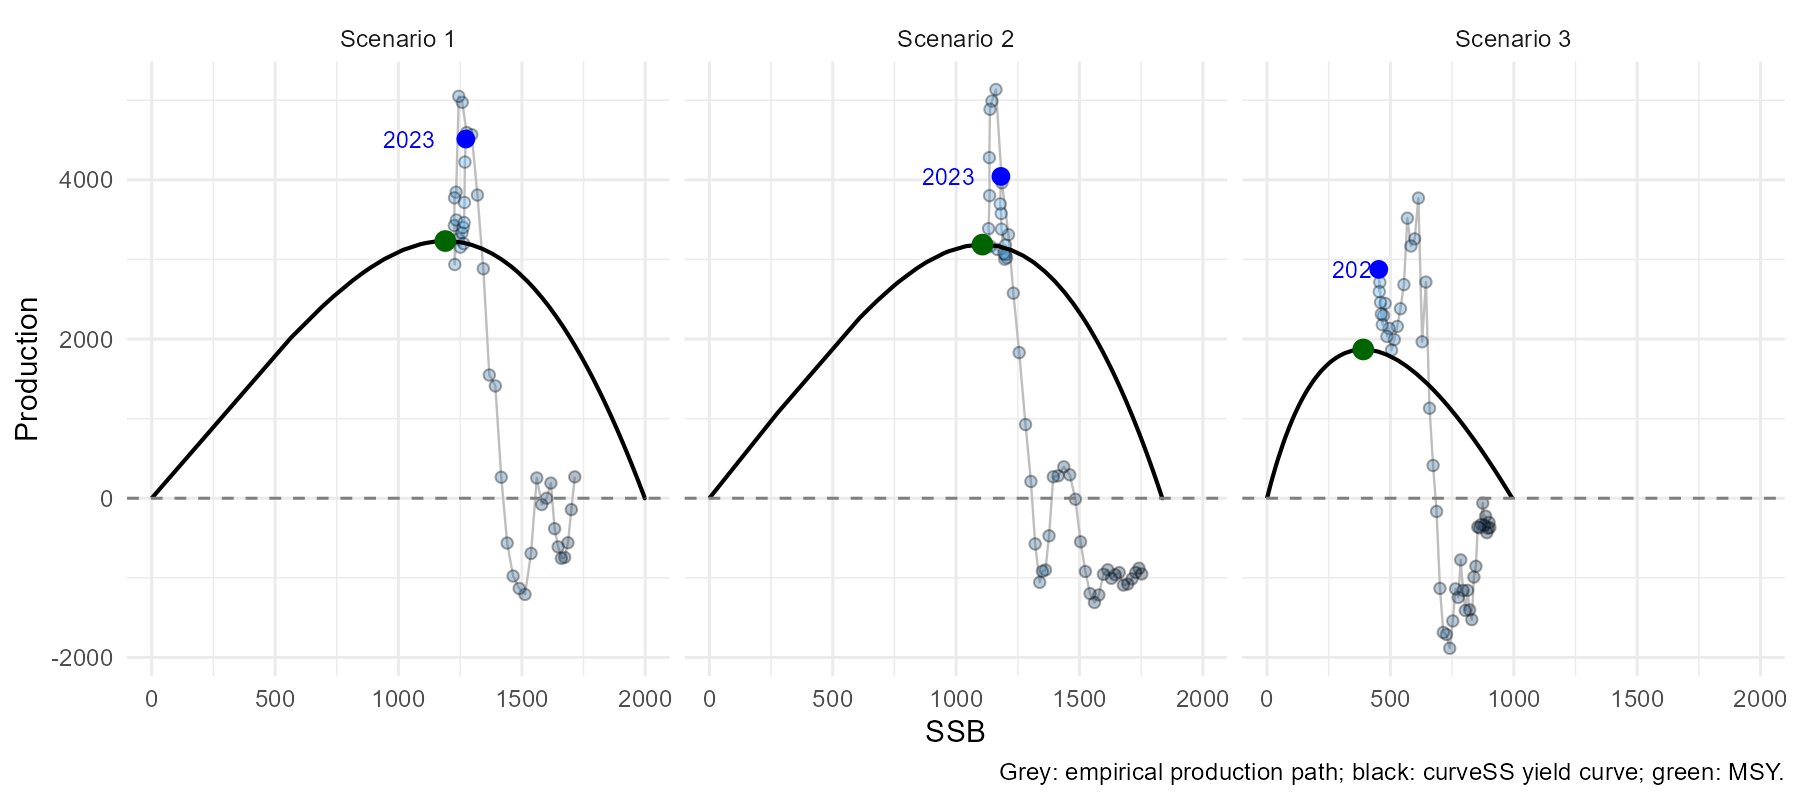
\includegraphics[width=0.92\linewidth]{figs/sma-fig-pe-phase-1.png}
  \caption{sma fig pe phase 1}
  \label{fig:internal-sma-fig-pe-phase-1}
\end{figure}

\begin{figure}[H]
  \centering
  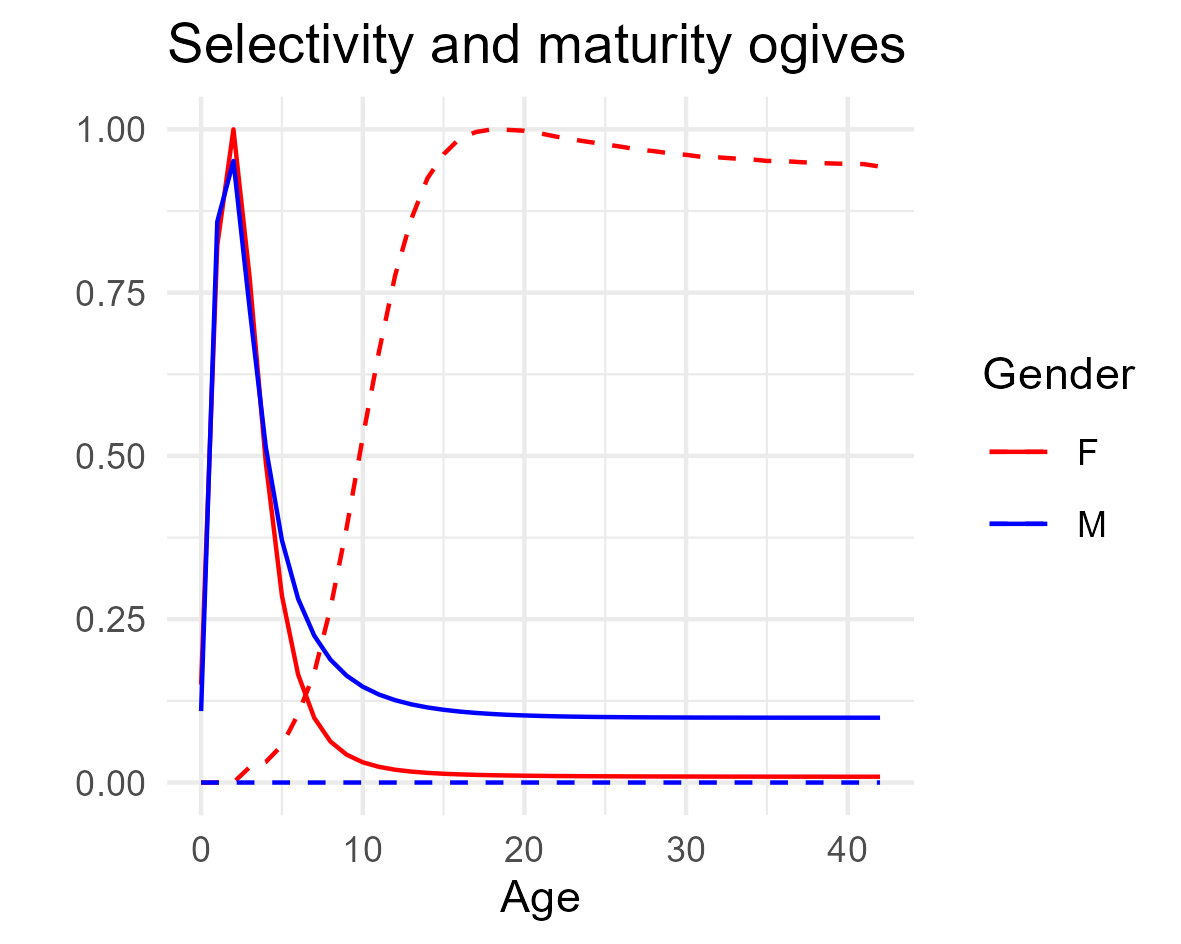
\includegraphics[width=0.92\linewidth]{figs/selmat.png}
  \caption{selmat}
  \label{fig:internal-selmat}
\end{figure}

\begin{figure}[H]
  \centering
  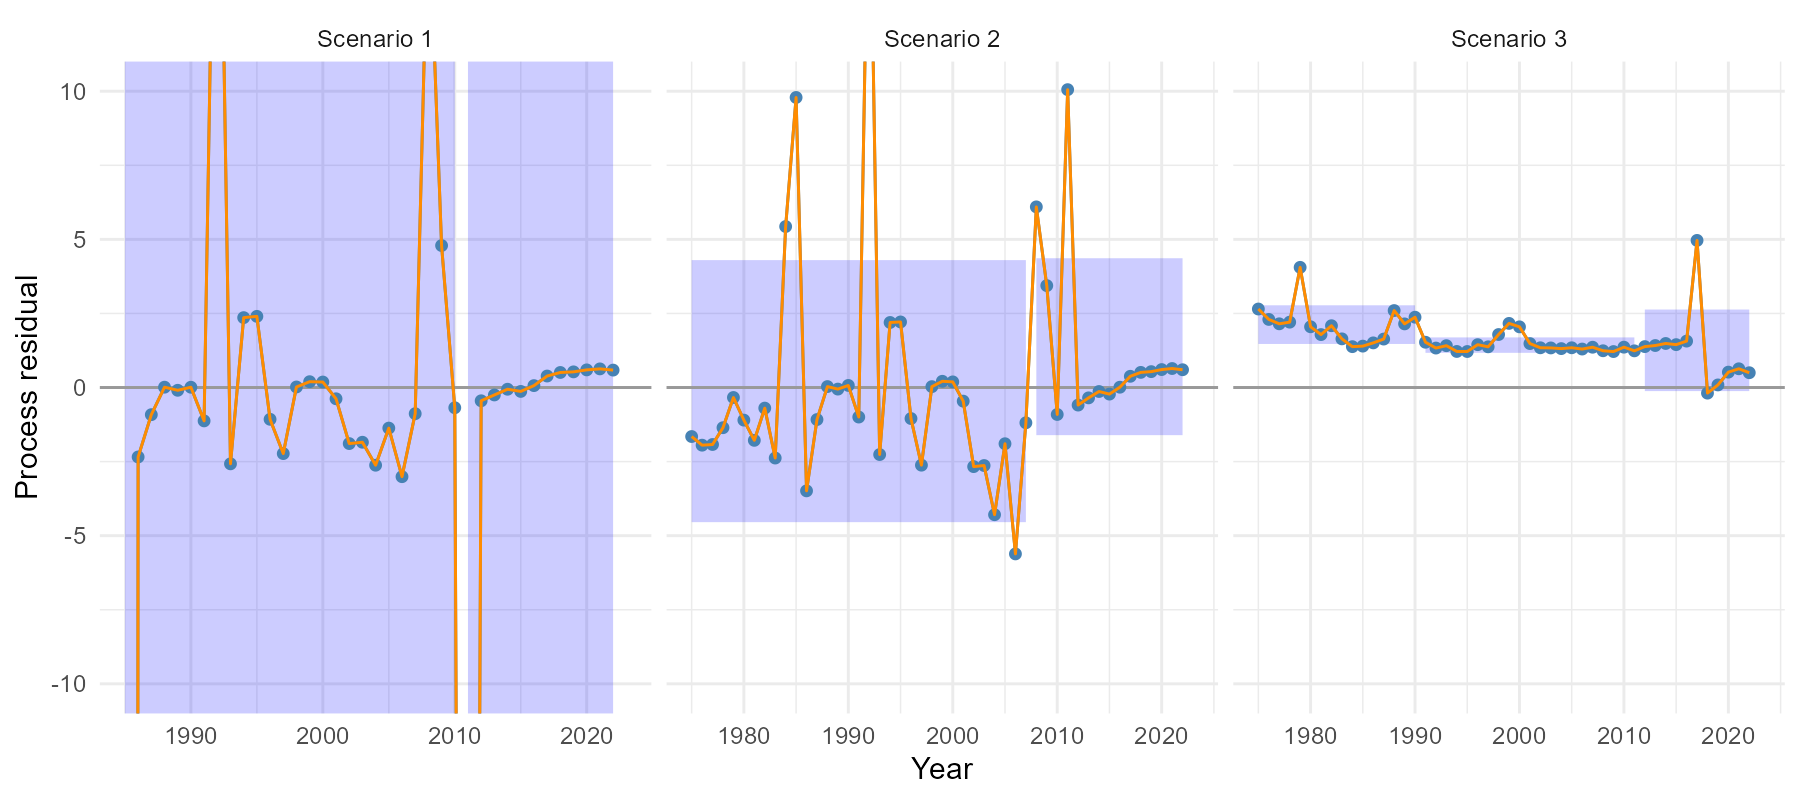
\includegraphics[width=0.92\linewidth]{figs/sma-fig-res-time-1.png}
  \caption{sma fig res time 1}
  \label{fig:internal-sma-fig-res-time-1}
\end{figure}

\begin{figure}[H]
  \centering
  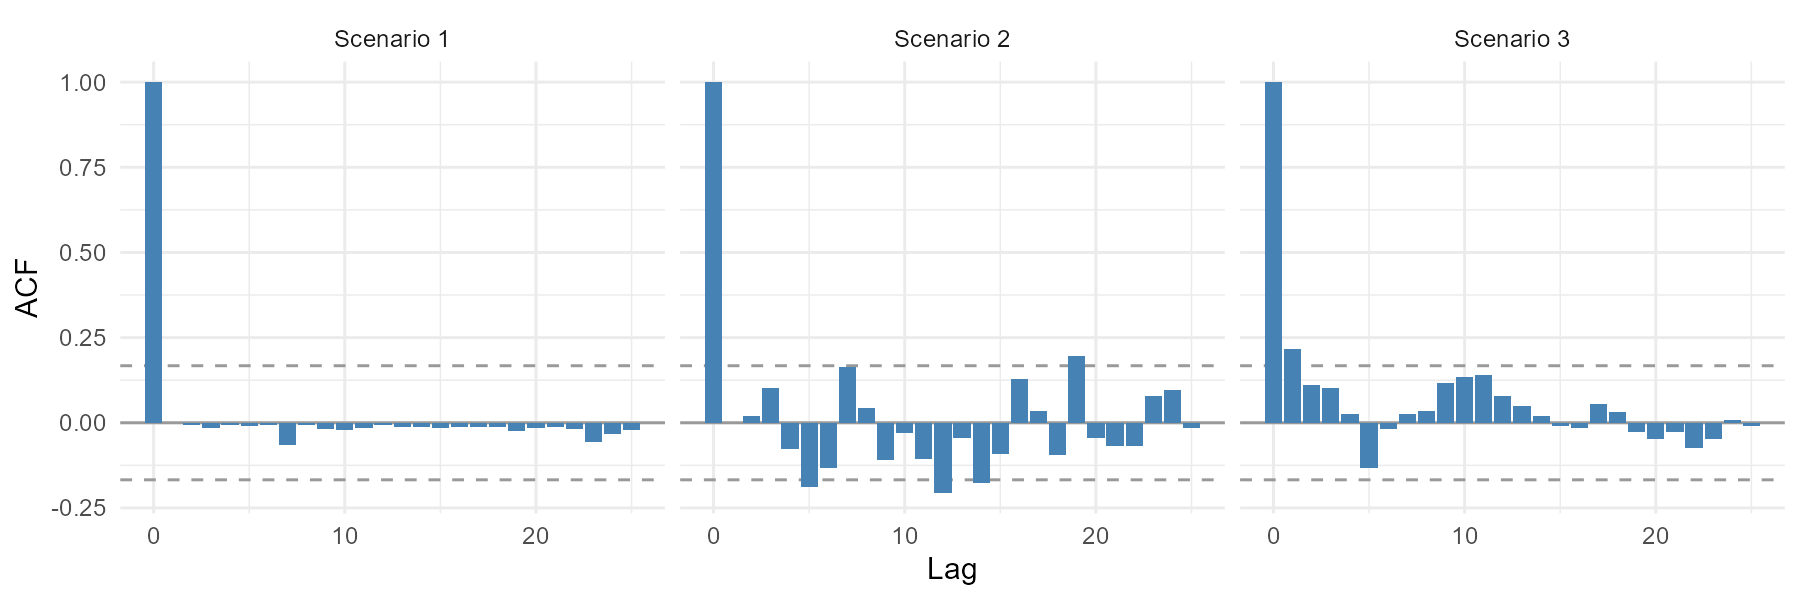
\includegraphics[width=0.92\linewidth]{figs/sma-fig-res-acf-1.png}
  \caption{sma fig res acf 1}
  \label{fig:internal-sma-fig-res-acf-1}
\end{figure}

\begin{figure}[H]
  \centering
  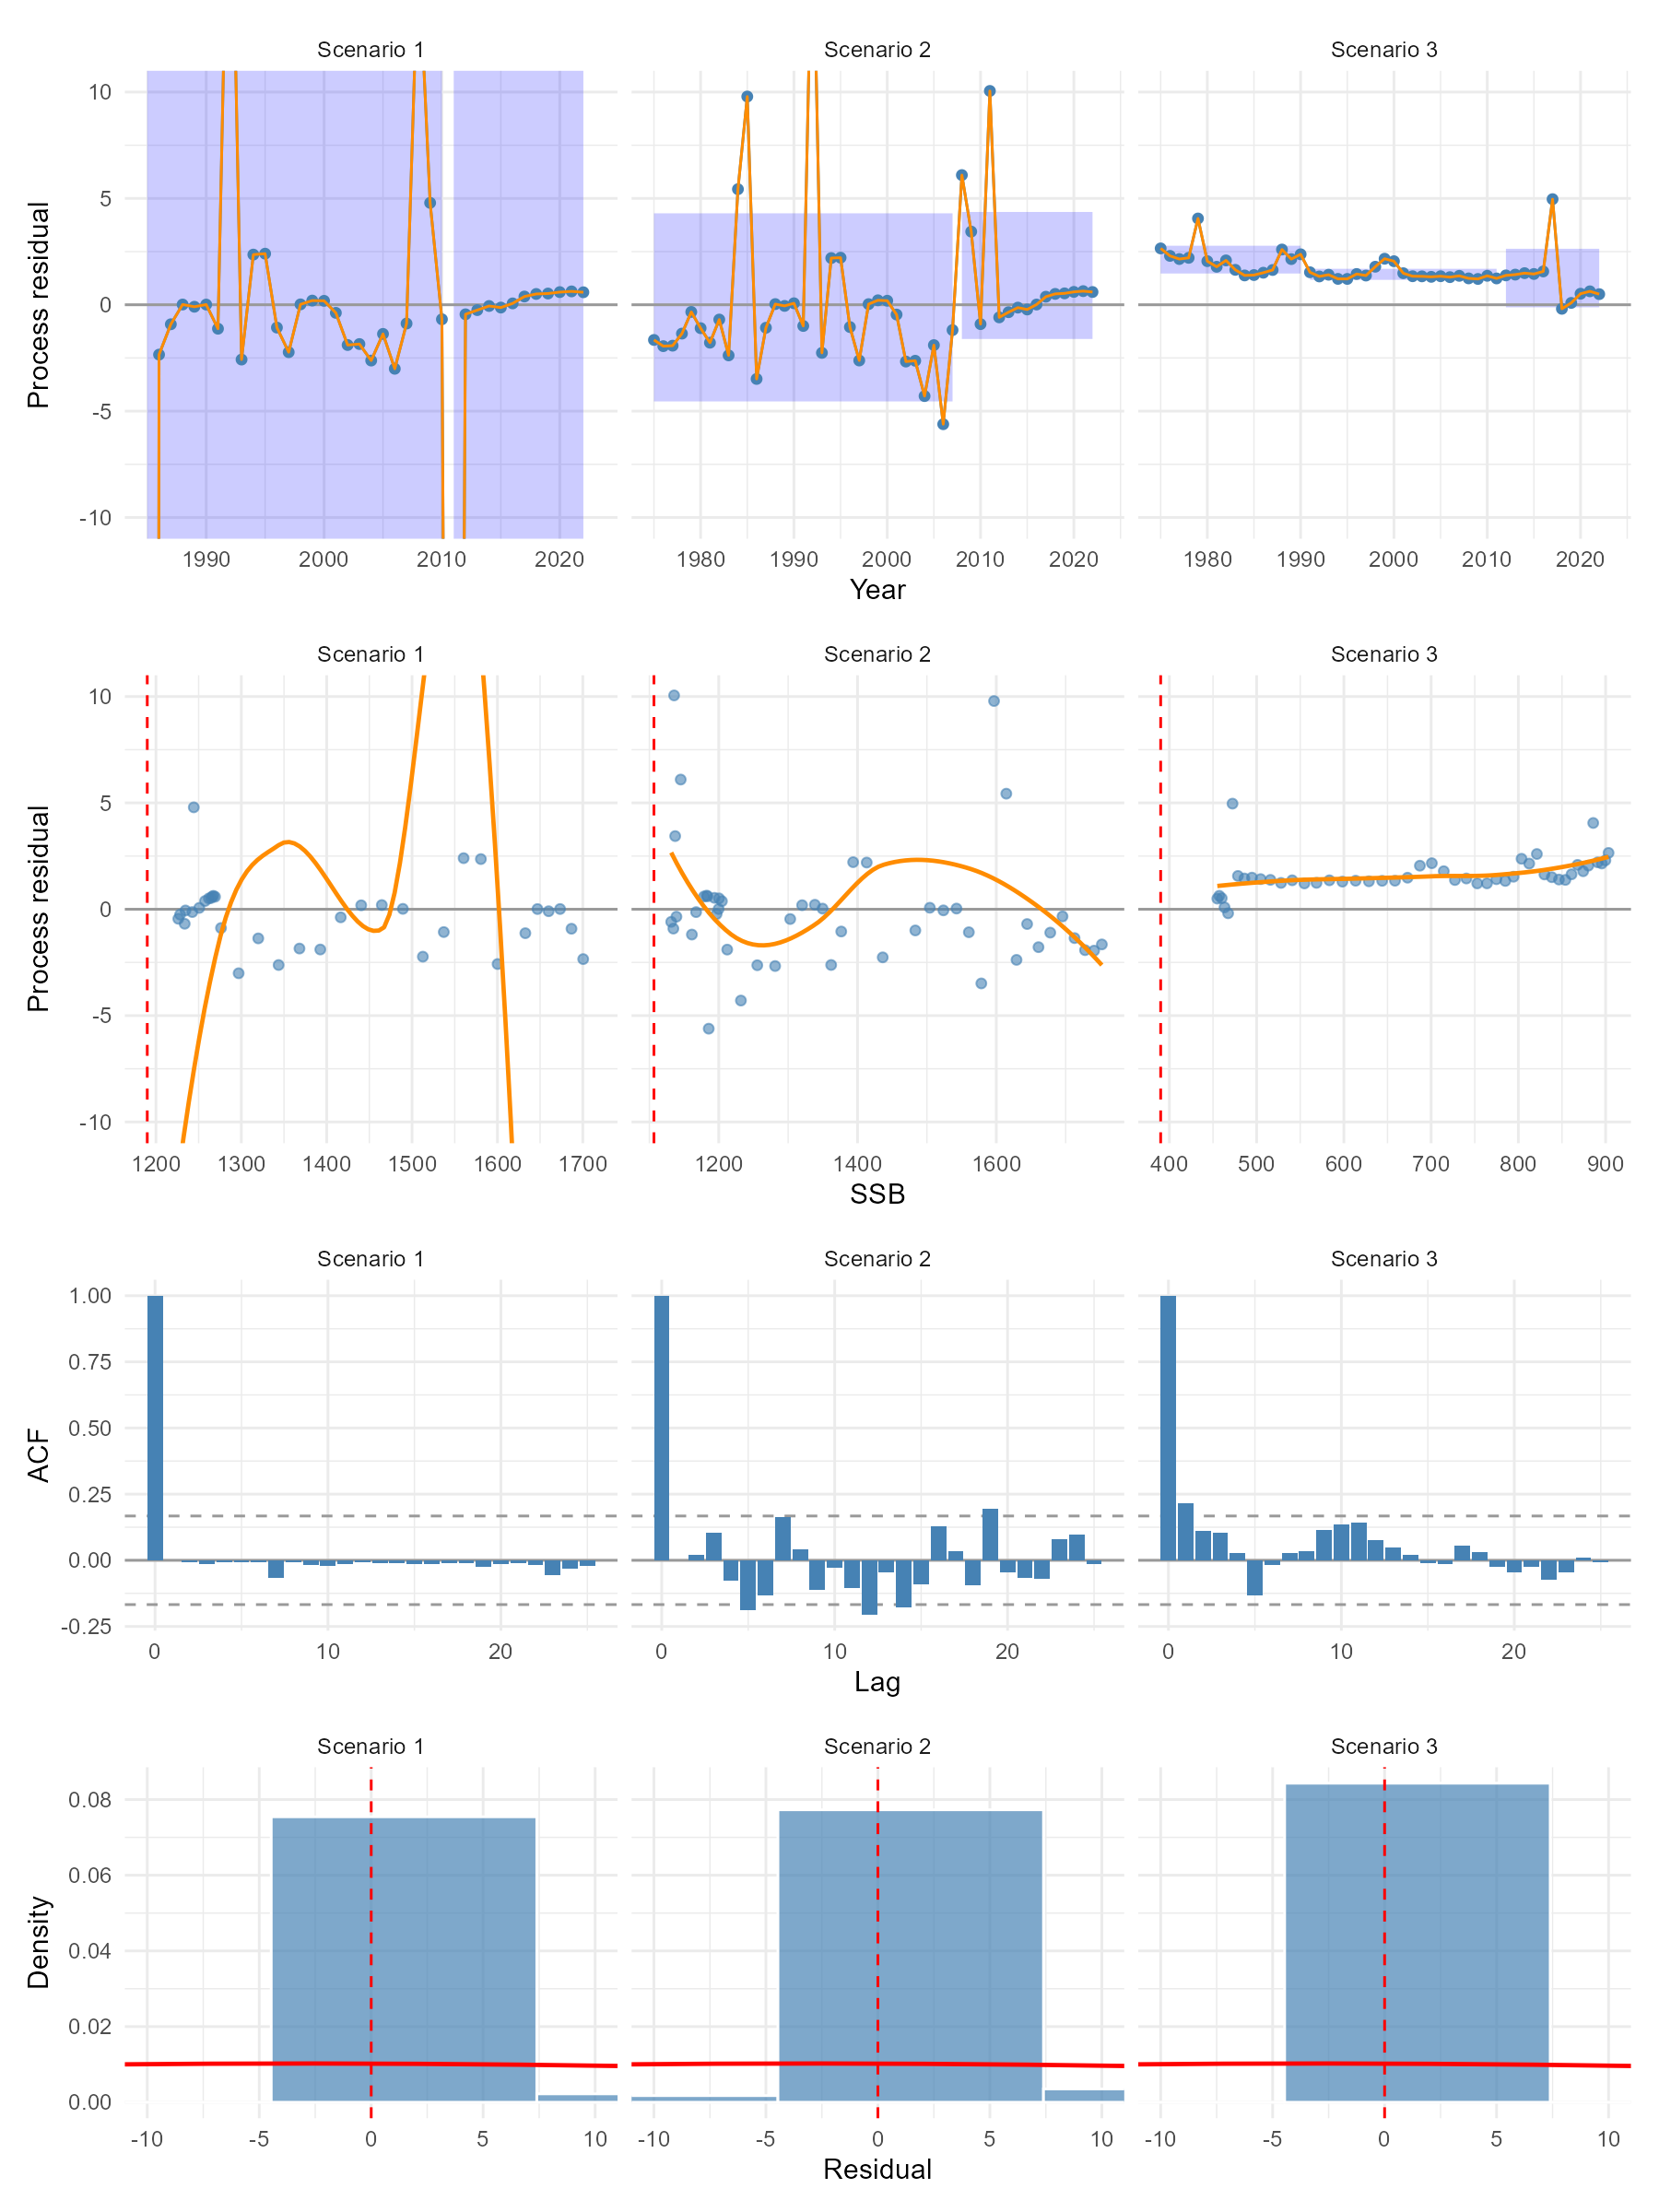
\includegraphics[width=0.92\linewidth]{figs/4panel.png}
  \caption{4panel}
  \label{fig:internal-4panel}
\end{figure}



\subsection{Interpretation}

Summarise whether the model is technically well fitted, which quantities are weakly
identified, and which issues should be carried forward to the robustness appendix.

% Case-specific internal interpretation.
% Summarise whether management quantities are informed by data,
% whether likelihood profiles or Hessian checks indicate weak identifiability,
% and which issues should be carried to the robustness appendix.



\section{External Diagnostics and Reproducible Workflow}
\label{app:external}

External diagnostics evaluate whether model outputs are consistent with specified
evidence outside the fitted likelihood. In this appendix, ``consistent'' should be
defined against explicit data sources or biological constraints, rather than by informal
judgement. Generic code for reading, plotting, and comparing indicators should live in
packages; case-study scripts should map model outputs to external evidence and write
results into the content files below.

\subsection{Required R Packages}

\begin{table}

\caption{\label{tab:external-libraries}Required R packages for external diagnostics.}
\centering
\begin{tabular}[t]{llll}
\toprule
package & role & tier & installed\\
\midrule
knitr & Knit template; format LaTeX tables & core & 1.51\\
r4ss & Read SS3 output for maturity, selectivity, and index fit & run\_code & 1.53.0\\
sstruth & diagSS, spSsbFromSs3, ssPeDiagnose; external CPUE and SP plots & run\_code & 0.0.0.9020\\
FLRebuild & curveSS(); production and reference points from SS3 & run\_code & 0.1.0\\
ss3om & readTruth / readFLSss3(); FLR stock objects from SS3 & run\_code & 0.5.3.9004\\
\addlinespace
FLCandy & matSel(); maturity vs selectivity ogives & run\_code & 1.7.1\\
diags & Extract CPUE/index series from SS3 diagnostics (.diagUss) & run\_code & 2.2.1\\
mpb & Lowess smoothing and scaling for CPUE time-series plots & run\_code & 3.5.0\\
plyr & Reshape index data (ddply) & run\_code & 1.8.9\\
reshape2 & Wide format for correlation plots (cast) & run\_code & 1.4.5\\
\addlinespace
ggplot2 & CPUE time series, survey vs biomass, sel/mat, LBI & run\_code & 4.0.3\\
GGally & Pairwise scatter plots of index correlations (planned) & planned & 2.4.0\\
ggcorrplot & Correlation matrix with hierarchical clustering (planned) & planned & 0.1.4.1\\
FLCore & FLR indicators and survey standardisation objects (planned) & planned & 2.6.29.9001\\
FLife & Cross-correlations between indices (planned) & planned & 3.4.0\\
\addlinespace
mydas & Life-history indicators (LBI); my\_smooth for ggpairs (planned) & planned & 1.2.2\\
\bottomrule
\end{tabular}
\end{table}



\subsection{Evidence Outside the Likelihood}

List the external evidence used in the case study:

\begin{itemize}
  \item life-history information, including growth, maturity, natural mortality, and longevity;
  \item fishery-independent survey trends, spatial indicators, and availability information;
  \item fishery behaviour, selectivity evidence, discard or bycatch information;
  \item environmental or ecosystem drivers already used in index standardisation;
  \item demographic indicators such as mature fraction, older-fish indicators, or age structure.
\end{itemize}

\begin{table}

\caption{\label{tab:external-evidence}External evidence register for the shortfin mako SS3 case study.}
\centering
\begin{tabular}[t]{lllll}
\toprule
diagnostic & evidence\_source & model\_quantity & criterion & status\\
\midrule
Growth and maturity & Life-history inputs to SS3 & Maturity-at-age vs selectivity-at-age & Fishing should not heavily precede 50 percent maturity on SSB scale & Check\\
Selectivity at age & Fleet selectivity ogives from SS3 & Selectivity ogive & Selectivity peak below maturity implies lagged SSB response & Mismatch flagged in case study\\
Survey perception & Standardised CPUE / survey indices (external to likelihood if pre-processed) & Index fit and scaling & Assessment trend coherent with survey perception & Check\\
Age structure & Length and age composition data & Age composition residuals & Older-fish / age-structure signals consistent with depletion narrative & Check\\
Spatial availability & Spatial models / availability (if used outside SS3) & Recruitment / availability deviations & No double-counting of spatial signal inside SS3 & Check\\
\addlinespace
Fishery behaviour / non-retention & Discard and non-retention regulations & Catch-at-age and discard mortality & Removals dominated by juveniles while state is mature female SSB & Mismatch flagged in case study\\
\bottomrule
\end{tabular}
\end{table}



\subsection{Standard Checks}

For SS3 and other age-structured assessments, useful external checks include maturity
versus selectivity, survey trend versus assessment biomass, spatial occupancy or aggregation
indicators, and comparison of recruitment or productivity regimes with external evidence.

% External comparison tables.

\begin{table}

\caption{\label{tab:external-sspe}Surplus-production vs SS3 process-error diagnostics (sstruth::ssPeDiagnose).}
\centering
\begin{tabular}[t]{lrrrrrrrl}
\toprule
scenario & curve\_cor & curve\_rmse & curve\_rel\_rmse & pe\_cor\_ssb & pe\_cor\_biomass & pe\_rmse\_ssb & pe\_rmse\_biomass & likely\_misspecified\\
\midrule
Scenario 1 & 0.9933 & 374.4 & 0.1159 & -0.2136 & 0.2427 & 7.196 & 0.006521 & TRUE\\
\bottomrule
\end{tabular}
\end{table}



\subsection{Diagnostic Output}

Tables, figures, and code-generated summaries can be added to the file below as they
become available.

% External diagnostic figures.

\begin{figure}[H]
  \centering
  \includegraphics[width=0.72\linewidth]{appendices/figs/external/cpue-ts.png}
  \caption{Standardised CPUE time series by fleet (sstruth::diagSS; lowess trend when mpb available).}
  \label{fig:external-cpue-ts}
\end{figure}

\begin{figure}[H]
  \centering
  \includegraphics[width=0.88\linewidth]{appendices/figs/external/sp-ssb.png}
  \caption{Empirical surplus production vs spawning stock biomass (sstruth::spSsbFromSs3).}
  \label{fig:external-sp-ssb}
\end{figure}

\begin{figure}[H]
  \centering
  \includegraphics[width=0.88\linewidth]{appendices/figs/external/selmat.png}
  \caption{Comparison of selectivity and maturity-at-age in the shortfin mako SS3 scenarios (from readFLSss3).}
  \label{fig:external-selmat}
\end{figure}



\subsection{Interpretation}

State which model outputs are consistent with external evidence, which are not, and which
external conflicts should be tested in the robustness appendix.

% Case-specific external interpretation.
% State which model outputs are consistent with life history and fishery evidence,
% which conflicts should be tested in the robustness appendix,
% and whether the biomass currency matches the age classes removed by fishing.



\section{Robustness Diagnostics and Reproducible Workflow}
\label{app:robustness}

Robustness diagnostics evaluate whether advice-relevant conclusions are stable under
pre-specified alternative structures. This appendix should separate estimation uncertainty
conditional on a reference model from sensitivity across models or scenarios. Generic
scenario comparison, hindcast, ensemble, and projection code should live in packages;
case-study scripts should define scenarios and write results into the content files below.

\subsection{Required R Packages}

\begin{table}

\caption{\label{tab:robustness-libraries}Required R packages for robustness diagnostics.}
\centering
\begin{tabular}[t]{llll}
\toprule
package & role & tier & installed\\
\midrule
knitr & Knit template; format LaTeX tables & core & 1.51\\
r4ss & Read SS3 output across scenarios & run\_code & 1.53.0\\
FLRebuild & curveSS(); scenario time series and process residuals & run\_code & 0.1.0\\
ss3om & readTruth / readFLSss3(); FLR stock objects from SS3 & run\_code & 0.5.3.9004\\
sstruth & retroBacktestData, plotRatios, ssPeDiagnose, plotSpSsb & run\_code & 0.0.0.9020\\
\addlinespace
ggplot2 & Scenario comparison, retrospective, and MVLN figures & run\_code & 4.0.3\\
dplyr & Retrospective trajectory plots (trajMsyLong); MVLN time-series summaries & run\_code & 1.2.1\\
plyr & Summarise scenario outputs (ddply) & run\_code & 1.8.9\\
reshape2 & Reshape scenario tables and MVLN draws (melt/cast) & run\_code & 1.4.5\\
tidyr & Reshape scenario and ensemble tables (planned) & planned & 1.3.2\\
\addlinespace
FLCore & FLR stock objects for status and reference points (planned) & planned & 2.6.29.9001\\
kobe & Kobe-phase plots (planned; ggplot used for MVLN Kobe comparison) & planned & 2.2.0\\
mvtnorm & Multivariate normal sampling for MVLN status uncertainty & run\_code & 1.3.3\\
patchwork & Combine MVLN status time-series panels (optional) & run\_code & 1.3.2\\
\bottomrule
\end{tabular}
\end{table}



\subsection{Scenario Register}

Each robustness appendix should begin with a scenario register. Scenarios should be
pre-specified before reviewing the results, and should identify which uncertainty source
they test.

\begin{table}

\caption{\label{tab:robustness-scenarios}Scenario register for robustness diagnostics (2026 ICCAT shark WG base runs).}
\centering
\begin{tabular}[t]{llllr}
\toprule
scenario & class & purpose & include\_in\_ensemble & weight\\
\midrule
Scenario 1 & reference & Reference assessment (Sc1\_Base) & TRUE & 0.3333333\\
Scenario 2 & structural sensitivity & Alternative structural assumption 1 (Scn02\_base) & TRUE & 0.3333333\\
Scenario 3 & structural sensitivity & Alternative structural assumption 2 (Sc3\_Base) & TRUE & 0.3333333\\
\bottomrule
\end{tabular}
\end{table}


\subsection{Standard Checks}

Robustness reporting should include:

\begin{itemize}
  \item retrospective patterns and hindcast or cross-validation prediction skill;
  \item alternative stock--recruitment, natural mortality, selectivity, catchability, or data-weighting structures;
  \item scenario or ensemble summaries for stock status, reference points, and catch advice;
  \item comparison of model error with estimation error from the reference case;
  \item central tendencies for target reference points and tail probabilities for limit reference points;
  \item rebuilding quantities such as $B_{\mathrm{rebuild}}$, $T_{\mathrm{rebuild}}$, and $P(\mathrm{rebuild\ within\ }T)$ where relevant;
  \item comparison of process-error diagnostics across model classes when ensembles combine biomass-dynamic (JABBA, SPiCT) and age-structured (SS3, SAM) formulations, using a common surplus-production currency on spawning biomass;
  \item hindcast and catch back-test forecast skill where retrospective peels are available.
\end{itemize}

% Robustness diagnostic checks.

\begin{table}

\caption{\label{tab:robustness-pe-summary}Terminal-year scenario status relative to MSY reference points (from curveSS).}
\centering
\begin{tabular}[t]{lrrrr}
\toprule
scenario & terminal\_year & ssb\_bmsy & catch\_msy & harvest\_fmsy\\
\midrule
Scenario 1 & 2023 & 1.07 & 0.429 & 0.401\\
Scenario 2 & 2023 & 1.07 & 0.436 & 0.408\\
Scenario 3 & 2023 & 1.16 & 0.742 & 0.639\\
\bottomrule
\end{tabular}
\end{table}

\begin{table}

\caption{\label{tab:robustness-sspe}Surplus-production misspecification flags by scenario (sstruth::ssPeDiagnose).}
\centering
\begin{tabular}[t]{lrrrrrrrl}
\toprule
scenario & curve\_cor & curve\_rmse & curve\_rel\_rmse & pe\_cor\_ssb & pe\_cor\_biomass & pe\_rmse\_ssb & pe\_rmse\_biomass & likely\_misspecified\\
\midrule
Scenario 1 & 0.9933 & 374.4 & 0.11590 & -0.21360 & 0.2427 & 7.196 & 0.006521 & TRUE\\
Scenario 2 & 0.9816 & 241.1 & 0.07565 & -0.06222 & -0.1129 & 16.800 & 0.007235 & TRUE\\
Scenario 3 & 0.9992 & 1200.0 & 0.64210 & 0.11780 & -0.2070 & 22.950 & 0.007739 & TRUE\\
\bottomrule
\end{tabular}
\end{table}

\begin{table}

\caption{\label{tab:robustness-retro-onestep}One-step-ahead retrospective errors (sstruth::retroBacktestData).}
\centering
\begin{tabular}[t]{llrrlrrrrrrrr}
\toprule
scenario & peel & terminalYr & forecastYr & baseRefEra & catchFore & forecastF & catchEstBaseTime & estFBaseTime & catchReportedData & relErrCatchVsEst & relErrFVsEst & relErrCatchVsReported\\
\midrule
Scenario-2 & 0 & 2023 & 2024 & FORE & 3497 & 0.18070 & 3497 & 0.1807 & 0 & 0.000000 & 0.000000 & NA\\
Scenario-2 & -1 & 2023 & 2024 & FORE & 3246 & 0.18230 & 3497 & 0.1807 & 0 & -0.071670 & 0.008362 & NA\\
Scenario-2 & -2 & 2023 & 2024 & FORE & 0 & 0.00000 & 3497 & 0.1807 & 0 & -1.000000 & -1.000000 & NA\\
Scenario-2 & -3 & 2023 & 2024 & FORE & 3582 & 0.19100 & 3497 & 0.1807 & 0 & 0.024420 & 0.056510 & NA\\
Scenario-2 & -4 & 2023 & 2024 & FORE & 3602 & 0.18690 & 3497 & 0.1807 & 0 & 0.030090 & 0.034030 & NA\\
\addlinespace
Scenario-2 & -5 & 2023 & 2024 & FORE & 3589 & 0.18030 & 3497 & 0.1807 & 0 & 0.026320 & -0.002669 & NA\\
Scenario-2 & -6 & 2023 & 2024 & FORE & 3577 & 0.17500 & 3497 & 0.1807 & 0 & 0.022840 & -0.032010 & NA\\
Scenario-2 & -7 & 2023 & 2024 & FORE & 3557 & 0.17460 & 3497 & 0.1807 & 0 & 0.017130 & -0.033830 & NA\\
Scenario-2 & -8 & 2023 & 2024 & FORE & 3470 & 0.17310 & 3497 & 0.1807 & 0 & -0.007715 & -0.042290 & NA\\
Scenario-2 & -9 & 2023 & 2024 & FORE & 3440 & 0.17280 & 3497 & 0.1807 & 0 & -0.016330 & -0.044060 & NA\\
\addlinespace
Scenario-2 & -10 & 2023 & 2024 & FORE & 3455 & 0.17330 & 3497 & 0.1807 & 0 & -0.011900 & -0.041230 & NA\\
Scenario-3 & 0 & 2023 & 2024 & FORE & 2056 & 0.08000 & 2056 & 0.0800 & 0 & 0.000000 & 0.000000 & NA\\
Scenario-3 & -1 & 2023 & 2024 & FORE & 0 & 0.00000 & 2056 & 0.0800 & 0 & -1.000000 & -1.000000 & NA\\
Scenario-3 & -2 & 2023 & 2024 & FORE & 1896 & 0.08577 & 2056 & 0.0800 & 0 & -0.077730 & 0.072210 & NA\\
Scenario-3 & -3 & 2023 & 2024 & FORE & 2032 & 0.08570 & 2056 & 0.0800 & 0 & -0.011440 & 0.071250 & NA\\
\addlinespace
Scenario-3 & -4 & 2023 & 2024 & FORE & 1927 & 0.08428 & 2056 & 0.0800 & 0 & -0.062570 & 0.053610 & NA\\
Scenario-3 & -5 & 2023 & 2024 & FORE & 1856 & 0.08289 & 2056 & 0.0800 & 0 & -0.097490 & 0.036150 & NA\\
Scenario-3 & -6 & 2023 & 2024 & FORE & 1780 & 0.08138 & 2056 & 0.0800 & 0 & -0.134400 & 0.017320 & NA\\
Scenario-3 & -7 & 2023 & 2024 & FORE & 1806 & 0.08284 & 2056 & 0.0800 & 0 & -0.121600 & 0.035590 & NA\\
Scenario-3 & -8 & 2023 & 2024 & FORE & 1722 & 0.08392 & 2056 & 0.0800 & 0 & -0.162600 & 0.049080 & NA\\
\addlinespace
Scenario-3 & -9 & 2023 & 2024 & FORE & 1542 & 0.08266 & 2056 & 0.0800 & 0 & -0.250200 & 0.033260 & NA\\
Scenario-3 & -10 & 2023 & 2024 & FORE & 1507 & 0.08584 & 2056 & 0.0800 & 0 & -0.267200 & 0.073090 & NA\\
\bottomrule
\end{tabular}
\end{table}

\begin{table}

\caption{\label{tab:robustness-mvln-terminal}Terminal-year MVLN status uncertainty by scenario (year 2023). Harvest = F/FMSY from Hessian draws.}
\centering
\begin{tabular}[t]{llrrrrrrrrrr}
\toprule
  & scenario & terminal\_year & stock\_median & stock\_p05 & stock\_p95 & harvest\_median & harvest\_p05 & harvest\_p95 & p\_overfished & p\_overfishing & weight\\
\midrule
Scenario-1 & Scenario-1 & 2023 & 1.05 & 0.867 & 1.32 & 24.3 & 21.0 & 27.9 & 0.326 & 1 & 0.333\\
Scenario-2 & Scenario-2 & 2023 & 1.06 & 0.926 & 1.22 & 25.4 & 23.1 & 28.1 & 0.220 & 1 & 0.333\\
Scenario-3 & Scenario-3 & 2023 & 1.16 & 0.938 & 1.42 & 43.3 & 35.5 & 52.7 & 0.112 & 1 & 0.333\\
\bottomrule
\end{tabular}
\end{table}

\begin{table}

\caption{\label{tab:robustness-catch-backtest}Catch back-test forecast summaries by peel and forecast scenario (collected via run-catch-backtests.R).}
\centering
\begin{tabular}[t]{lllrrrrll}
\toprule
scenario & peel & forecast\_scenario & forecast\_year & spawn\_bio & dead\_catch & sum\_f & run\_dir & ok\\
\midrule
Scenario-2 & 0 & catchReported & 2024 & 1188.0 & NA & NA & C:/active/flr/sstruth/data/ss3/sma-natl/Scenario-2/retrospectives/retro0/catchReported & TRUE\\
Scenario-2 & 0 & fMeanFull & 2024 & 1188.0 & NA & NA & C:/active/flr/sstruth/data/ss3/sma-natl/Scenario-2/retrospectives/retro0/fMeanFull & TRUE\\
Scenario-2 & 0 & fZero & 2024 & 1188.0 & NA & NA & C:/active/flr/sstruth/data/ss3/sma-natl/Scenario-2/retrospectives/retro0/fZero & TRUE\\
Scenario-2 & 0 & fMsy & 2024 & 1188.0 & NA & NA & C:/active/flr/sstruth/data/ss3/sma-natl/Scenario-2/retrospectives/retro0/fMsy & TRUE\\
Scenario-2 & -1 & catchReported & 2024 & 1184.0 & NA & NA & C:/active/flr/sstruth/data/ss3/sma-natl/Scenario-2/retrospectives/retro-1/catchReported & TRUE\\
\addlinespace
Scenario-2 & -1 & fMeanFull & 2024 & 1184.0 & NA & NA & C:/active/flr/sstruth/data/ss3/sma-natl/Scenario-2/retrospectives/retro-1/fMeanFull & TRUE\\
Scenario-2 & -1 & fZero & 2024 & 1184.0 & NA & NA & C:/active/flr/sstruth/data/ss3/sma-natl/Scenario-2/retrospectives/retro-1/fZero & TRUE\\
Scenario-2 & -1 & fMsy & 2024 & 1184.0 & NA & NA & C:/active/flr/sstruth/data/ss3/sma-natl/Scenario-2/retrospectives/retro-1/fMsy & TRUE\\
Scenario-2 & -2 & catchReported & 2024 & 1243.0 & NA & NA & C:/active/flr/sstruth/data/ss3/sma-natl/Scenario-2/retrospectives/retro-2/catchReported & TRUE\\
Scenario-2 & -2 & fMeanFull & 2024 & 1243.0 & NA & NA & C:/active/flr/sstruth/data/ss3/sma-natl/Scenario-2/retrospectives/retro-2/fMeanFull & TRUE\\
\addlinespace
Scenario-2 & -2 & fZero & 2024 & 1243.0 & NA & NA & C:/active/flr/sstruth/data/ss3/sma-natl/Scenario-2/retrospectives/retro-2/fZero & TRUE\\
Scenario-2 & -2 & fMsy & 2024 & 1243.0 & NA & NA & C:/active/flr/sstruth/data/ss3/sma-natl/Scenario-2/retrospectives/retro-2/fMsy & TRUE\\
Scenario-2 & -3 & catchReported & 2024 & 1252.0 & NA & NA & C:/active/flr/sstruth/data/ss3/sma-natl/Scenario-2/retrospectives/retro-3/catchReported & TRUE\\
Scenario-2 & -3 & fMeanFull & 2024 & 1252.0 & NA & NA & C:/active/flr/sstruth/data/ss3/sma-natl/Scenario-2/retrospectives/retro-3/fMeanFull & TRUE\\
Scenario-2 & -3 & fZero & 2024 & 1252.0 & NA & NA & C:/active/flr/sstruth/data/ss3/sma-natl/Scenario-2/retrospectives/retro-3/fZero & TRUE\\
\addlinespace
Scenario-2 & -3 & fMsy & 2024 & 1252.0 & NA & NA & C:/active/flr/sstruth/data/ss3/sma-natl/Scenario-2/retrospectives/retro-3/fMsy & TRUE\\
Scenario-2 & -4 & catchReported & 2024 & 1238.0 & NA & NA & C:/active/flr/sstruth/data/ss3/sma-natl/Scenario-2/retrospectives/retro-4/catchReported & TRUE\\
Scenario-2 & -4 & fMeanFull & 2024 & 1238.0 & NA & NA & C:/active/flr/sstruth/data/ss3/sma-natl/Scenario-2/retrospectives/retro-4/fMeanFull & TRUE\\
Scenario-2 & -4 & fZero & 2024 & 1238.0 & NA & NA & C:/active/flr/sstruth/data/ss3/sma-natl/Scenario-2/retrospectives/retro-4/fZero & TRUE\\
Scenario-2 & -4 & fMsy & 2024 & 1238.0 & NA & NA & C:/active/flr/sstruth/data/ss3/sma-natl/Scenario-2/retrospectives/retro-4/fMsy & TRUE\\
\addlinespace
Scenario-2 & -5 & catchReported & 2024 & 1203.0 & NA & NA & C:/active/flr/sstruth/data/ss3/sma-natl/Scenario-2/retrospectives/retro-5/catchReported & TRUE\\
Scenario-2 & -5 & fMeanFull & 2024 & 1203.0 & NA & NA & C:/active/flr/sstruth/data/ss3/sma-natl/Scenario-2/retrospectives/retro-5/fMeanFull & TRUE\\
Scenario-2 & -5 & fZero & 2024 & 1203.0 & NA & NA & C:/active/flr/sstruth/data/ss3/sma-natl/Scenario-2/retrospectives/retro-5/fZero & TRUE\\
Scenario-2 & -5 & fMsy & 2024 & 1203.0 & NA & NA & C:/active/flr/sstruth/data/ss3/sma-natl/Scenario-2/retrospectives/retro-5/fMsy & TRUE\\
Scenario-2 & -6 & catchReported & 2024 & 1196.0 & NA & NA & C:/active/flr/sstruth/data/ss3/sma-natl/Scenario-2/retrospectives/retro-6/catchReported & TRUE\\
\addlinespace
Scenario-2 & -6 & fMeanFull & 2024 & 1196.0 & NA & NA & C:/active/flr/sstruth/data/ss3/sma-natl/Scenario-2/retrospectives/retro-6/fMeanFull & TRUE\\
Scenario-2 & -6 & fZero & 2024 & 1196.0 & NA & NA & C:/active/flr/sstruth/data/ss3/sma-natl/Scenario-2/retrospectives/retro-6/fZero & TRUE\\
Scenario-2 & -6 & fMsy & 2024 & 1196.0 & NA & NA & C:/active/flr/sstruth/data/ss3/sma-natl/Scenario-2/retrospectives/retro-6/fMsy & TRUE\\
Scenario-2 & -7 & catchReported & 2024 & 1160.0 & NA & NA & C:/active/flr/sstruth/data/ss3/sma-natl/Scenario-2/retrospectives/retro-7/catchReported & TRUE\\
Scenario-2 & -7 & fMeanFull & 2024 & 1160.0 & NA & NA & C:/active/flr/sstruth/data/ss3/sma-natl/Scenario-2/retrospectives/retro-7/fMeanFull & TRUE\\
\addlinespace
Scenario-2 & -7 & fZero & 2024 & 1160.0 & NA & NA & C:/active/flr/sstruth/data/ss3/sma-natl/Scenario-2/retrospectives/retro-7/fZero & TRUE\\
Scenario-2 & -7 & fMsy & 2024 & 1160.0 & NA & NA & C:/active/flr/sstruth/data/ss3/sma-natl/Scenario-2/retrospectives/retro-7/fMsy & TRUE\\
Scenario-2 & -8 & catchReported & 2024 & 1116.0 & NA & NA & C:/active/flr/sstruth/data/ss3/sma-natl/Scenario-2/retrospectives/retro-8/catchReported & TRUE\\
Scenario-2 & -8 & fMeanFull & 2024 & 1116.0 & NA & NA & C:/active/flr/sstruth/data/ss3/sma-natl/Scenario-2/retrospectives/retro-8/fMeanFull & TRUE\\
Scenario-2 & -8 & fZero & 2024 & 1116.0 & NA & NA & C:/active/flr/sstruth/data/ss3/sma-natl/Scenario-2/retrospectives/retro-8/fZero & TRUE\\
\addlinespace
Scenario-2 & -8 & fMsy & 2024 & 1116.0 & NA & NA & C:/active/flr/sstruth/data/ss3/sma-natl/Scenario-2/retrospectives/retro-8/fMsy & TRUE\\
Scenario-2 & -9 & catchReported & 2024 & 1089.0 & NA & NA & C:/active/flr/sstruth/data/ss3/sma-natl/Scenario-2/retrospectives/retro-9/catchReported & TRUE\\
Scenario-2 & -9 & fMeanFull & 2024 & 1089.0 & NA & NA & C:/active/flr/sstruth/data/ss3/sma-natl/Scenario-2/retrospectives/retro-9/fMeanFull & TRUE\\
Scenario-2 & -9 & fZero & 2024 & 1089.0 & NA & NA & C:/active/flr/sstruth/data/ss3/sma-natl/Scenario-2/retrospectives/retro-9/fZero & TRUE\\
Scenario-2 & -9 & fMsy & 2024 & 1089.0 & NA & NA & C:/active/flr/sstruth/data/ss3/sma-natl/Scenario-2/retrospectives/retro-9/fMsy & TRUE\\
\addlinespace
Scenario-2 & -10 & catchReported & 2024 & 1079.0 & NA & NA & C:/active/flr/sstruth/data/ss3/sma-natl/Scenario-2/retrospectives/retro-10/catchReported & TRUE\\
Scenario-2 & -10 & fMeanFull & 2024 & 1079.0 & NA & NA & C:/active/flr/sstruth/data/ss3/sma-natl/Scenario-2/retrospectives/retro-10/fMeanFull & TRUE\\
Scenario-2 & -10 & fZero & 2024 & 1079.0 & NA & NA & C:/active/flr/sstruth/data/ss3/sma-natl/Scenario-2/retrospectives/retro-10/fZero & TRUE\\
Scenario-2 & -10 & fMsy & 2024 & 1079.0 & NA & NA & C:/active/flr/sstruth/data/ss3/sma-natl/Scenario-2/retrospectives/retro-10/fMsy & TRUE\\
Scenario-3 & 0 & catchReported & 2024 & 451.1 & NA & NA & C:/active/flr/sstruth/data/ss3/sma-natl/Scenario-3/retrospectives/retro0/catchReported & TRUE\\
\addlinespace
Scenario-3 & 0 & fMeanFull & 2024 & 451.1 & NA & NA & C:/active/flr/sstruth/data/ss3/sma-natl/Scenario-3/retrospectives/retro0/fMeanFull & TRUE\\
Scenario-3 & 0 & fZero & 2024 & 451.1 & NA & NA & C:/active/flr/sstruth/data/ss3/sma-natl/Scenario-3/retrospectives/retro0/fZero & TRUE\\
Scenario-3 & 0 & fMsy & 2024 & 451.1 & NA & NA & C:/active/flr/sstruth/data/ss3/sma-natl/Scenario-3/retrospectives/retro0/fMsy & TRUE\\
Scenario-3 & -1 & catchReported & 2024 & 447.3 & NA & NA & C:/active/flr/sstruth/data/ss3/sma-natl/Scenario-3/retrospectives/retro-1/catchReported & TRUE\\
Scenario-3 & -1 & fMeanFull & 2024 & 447.3 & NA & NA & C:/active/flr/sstruth/data/ss3/sma-natl/Scenario-3/retrospectives/retro-1/fMeanFull & TRUE\\
\addlinespace
Scenario-3 & -1 & fZero & 2024 & 447.3 & NA & NA & C:/active/flr/sstruth/data/ss3/sma-natl/Scenario-3/retrospectives/retro-1/fZero & TRUE\\
Scenario-3 & -1 & fMsy & 2024 & 447.3 & NA & NA & C:/active/flr/sstruth/data/ss3/sma-natl/Scenario-3/retrospectives/retro-1/fMsy & TRUE\\
Scenario-3 & -2 & catchReported & 2024 & 472.4 & NA & NA & C:/active/flr/sstruth/data/ss3/sma-natl/Scenario-3/retrospectives/retro-2/catchReported & TRUE\\
Scenario-3 & -2 & fMeanFull & 2024 & 472.4 & NA & NA & C:/active/flr/sstruth/data/ss3/sma-natl/Scenario-3/retrospectives/retro-2/fMeanFull & TRUE\\
Scenario-3 & -2 & fZero & 2024 & 472.4 & NA & NA & C:/active/flr/sstruth/data/ss3/sma-natl/Scenario-3/retrospectives/retro-2/fZero & TRUE\\
\addlinespace
Scenario-3 & -2 & fMsy & 2024 & 472.4 & NA & NA & C:/active/flr/sstruth/data/ss3/sma-natl/Scenario-3/retrospectives/retro-2/fMsy & TRUE\\
Scenario-3 & -3 & catchReported & 2024 & 471.4 & NA & NA & C:/active/flr/sstruth/data/ss3/sma-natl/Scenario-3/retrospectives/retro-3/catchReported & TRUE\\
Scenario-3 & -3 & fMeanFull & 2024 & 471.4 & NA & NA & C:/active/flr/sstruth/data/ss3/sma-natl/Scenario-3/retrospectives/retro-3/fMeanFull & TRUE\\
Scenario-3 & -3 & fZero & 2024 & 471.4 & NA & NA & C:/active/flr/sstruth/data/ss3/sma-natl/Scenario-3/retrospectives/retro-3/fZero & TRUE\\
Scenario-3 & -3 & fMsy & 2024 & 471.4 & NA & NA & C:/active/flr/sstruth/data/ss3/sma-natl/Scenario-3/retrospectives/retro-3/fMsy & TRUE\\
\addlinespace
Scenario-3 & -4 & catchReported & 2024 & 463.6 & NA & NA & C:/active/flr/sstruth/data/ss3/sma-natl/Scenario-3/retrospectives/retro-4/catchReported & TRUE\\
Scenario-3 & -4 & fMeanFull & 2024 & 463.6 & NA & NA & C:/active/flr/sstruth/data/ss3/sma-natl/Scenario-3/retrospectives/retro-4/fMeanFull & TRUE\\
Scenario-3 & -4 & fZero & 2024 & 463.6 & NA & NA & C:/active/flr/sstruth/data/ss3/sma-natl/Scenario-3/retrospectives/retro-4/fZero & TRUE\\
Scenario-3 & -4 & fMsy & 2024 & 463.6 & NA & NA & C:/active/flr/sstruth/data/ss3/sma-natl/Scenario-3/retrospectives/retro-4/fMsy & TRUE\\
Scenario-3 & -5 & catchReported & 2024 & 448.2 & NA & NA & C:/active/flr/sstruth/data/ss3/sma-natl/Scenario-3/retrospectives/retro-5/catchReported & TRUE\\
\addlinespace
Scenario-3 & -5 & fMeanFull & 2024 & 448.2 & NA & NA & C:/active/flr/sstruth/data/ss3/sma-natl/Scenario-3/retrospectives/retro-5/fMeanFull & TRUE\\
Scenario-3 & -5 & fZero & 2024 & 448.2 & NA & NA & C:/active/flr/sstruth/data/ss3/sma-natl/Scenario-3/retrospectives/retro-5/fZero & TRUE\\
Scenario-3 & -5 & fMsy & 2024 & 448.2 & NA & NA & C:/active/flr/sstruth/data/ss3/sma-natl/Scenario-3/retrospectives/retro-5/fMsy & TRUE\\
Scenario-3 & -6 & catchReported & 2024 & 436.5 & NA & NA & C:/active/flr/sstruth/data/ss3/sma-natl/Scenario-3/retrospectives/retro-6/catchReported & TRUE\\
Scenario-3 & -6 & fMeanFull & 2024 & 436.5 & NA & NA & C:/active/flr/sstruth/data/ss3/sma-natl/Scenario-3/retrospectives/retro-6/fMeanFull & TRUE\\
\addlinespace
Scenario-3 & -6 & fZero & 2024 & 436.5 & NA & NA & C:/active/flr/sstruth/data/ss3/sma-natl/Scenario-3/retrospectives/retro-6/fZero & TRUE\\
Scenario-3 & -6 & fMsy & 2024 & 436.5 & NA & NA & C:/active/flr/sstruth/data/ss3/sma-natl/Scenario-3/retrospectives/retro-6/fMsy & TRUE\\
Scenario-3 & -7 & catchReported & 2024 & 435.6 & NA & NA & C:/active/flr/sstruth/data/ss3/sma-natl/Scenario-3/retrospectives/retro-7/catchReported & TRUE\\
Scenario-3 & -7 & fMeanFull & 2024 & 435.6 & NA & NA & C:/active/flr/sstruth/data/ss3/sma-natl/Scenario-3/retrospectives/retro-7/fMeanFull & TRUE\\
Scenario-3 & -7 & fZero & 2024 & 435.6 & NA & NA & C:/active/flr/sstruth/data/ss3/sma-natl/Scenario-3/retrospectives/retro-7/fZero & TRUE\\
\addlinespace
Scenario-3 & -7 & fMsy & 2024 & 435.6 & NA & NA & C:/active/flr/sstruth/data/ss3/sma-natl/Scenario-3/retrospectives/retro-7/fMsy & TRUE\\
Scenario-3 & -8 & catchReported & 2024 & 415.5 & NA & NA & C:/active/flr/sstruth/data/ss3/sma-natl/Scenario-3/retrospectives/retro-8/catchReported & TRUE\\
Scenario-3 & -8 & fMeanFull & 2024 & 415.5 & NA & NA & C:/active/flr/sstruth/data/ss3/sma-natl/Scenario-3/retrospectives/retro-8/fMeanFull & TRUE\\
Scenario-3 & -8 & fZero & 2024 & 415.5 & NA & NA & C:/active/flr/sstruth/data/ss3/sma-natl/Scenario-3/retrospectives/retro-8/fZero & TRUE\\
Scenario-3 & -8 & fMsy & 2024 & 415.5 & NA & NA & C:/active/flr/sstruth/data/ss3/sma-natl/Scenario-3/retrospectives/retro-8/fMsy & TRUE\\
\addlinespace
Scenario-3 & -9 & catchReported & 2024 & 380.5 & NA & NA & C:/active/flr/sstruth/data/ss3/sma-natl/Scenario-3/retrospectives/retro-9/catchReported & TRUE\\
Scenario-3 & -9 & fMeanFull & 2024 & 380.5 & NA & NA & C:/active/flr/sstruth/data/ss3/sma-natl/Scenario-3/retrospectives/retro-9/fMeanFull & TRUE\\
Scenario-3 & -9 & fZero & 2024 & 380.5 & NA & NA & C:/active/flr/sstruth/data/ss3/sma-natl/Scenario-3/retrospectives/retro-9/fZero & TRUE\\
Scenario-3 & -9 & fMsy & 2024 & 380.5 & NA & NA & C:/active/flr/sstruth/data/ss3/sma-natl/Scenario-3/retrospectives/retro-9/fMsy & TRUE\\
Scenario-3 & -10 & catchReported & 2024 & 356.2 & NA & NA & C:/active/flr/sstruth/data/ss3/sma-natl/Scenario-3/retrospectives/retro-10/catchReported & TRUE\\
\addlinespace
Scenario-3 & -10 & fMeanFull & 2024 & 356.2 & NA & NA & C:/active/flr/sstruth/data/ss3/sma-natl/Scenario-3/retrospectives/retro-10/fMeanFull & TRUE\\
Scenario-3 & -10 & fZero & 2024 & 356.2 & NA & NA & C:/active/flr/sstruth/data/ss3/sma-natl/Scenario-3/retrospectives/retro-10/fZero & TRUE\\
Scenario-3 & -10 & fMsy & 2024 & 356.2 & NA & NA & C:/active/flr/sstruth/data/ss3/sma-natl/Scenario-3/retrospectives/retro-10/fMsy & TRUE\\
\bottomrule
\end{tabular}
\end{table}



\subsection{Diagnostic Output}

Tables, figures, and code-generated summaries can be added to the file below as they
become available.

% Robustness diagnostic figures.

\begin{figure}[H]
  \centering
  \includegraphics[width=0.92\linewidth]{appendices/figs/robustness/ss3-ts.png}
  \caption{SS3 scenario time series relative to MSY reference points.}
  \label{fig:robustness-ss3-ts}
\end{figure}

\begin{figure}[H]
  \centering
  \includegraphics[width=0.92\linewidth]{appendices/figs/robustness/ss3-res-time.png}
  \caption{Process residuals by scenario (from curveSS).}
  \label{fig:robustness-ss3-res-time}
\end{figure}

\begin{figure}[H]
  \centering
  \includegraphics[width=0.92\linewidth]{appendices/figs/robustness/ss3-res-acf.png}
  \caption{ACF of process residuals by scenario.}
  \label{fig:robustness-ss3-res-acf}
\end{figure}

\begin{figure}[H]
  \centering
  \includegraphics[width=0.95\linewidth]{appendices/figs/robustness/retro-traj-msy.png}
  \caption{Retrospective peel trajectories vs MSY benchmarks (sstruth::retroBacktestData).}
  \label{fig:robustness-retro-traj}
\end{figure}

\begin{figure}[H]
  \centering
  \includegraphics[width=0.92\linewidth]{appendices/figs/robustness/retro-bratio-horizon.png}
  \caption{Multi-horizon SSB/BMSY retrospective ratios (sstruth::plotRatios).}
  \label{fig:robustness-retro-bratio}
\end{figure}

\begin{figure}[H]
  \centering
  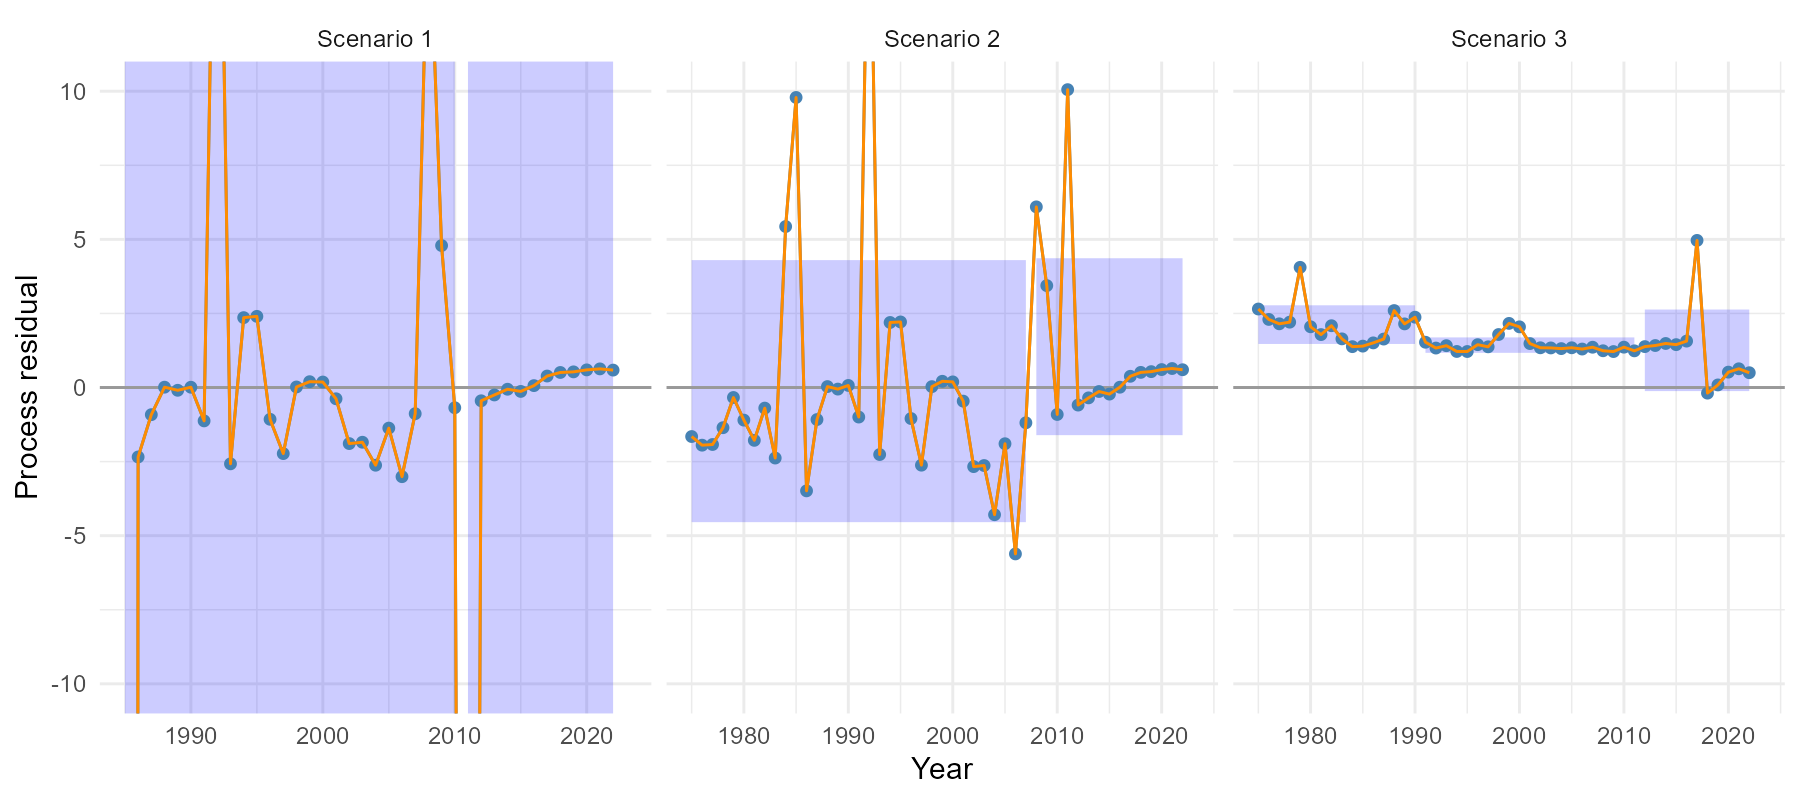
\includegraphics[width=0.92\linewidth]{figs/sma-fig-res-time-1.png}
  \caption{sma fig res time 1}
  \label{fig:robustness-sma-fig-res-time-1}
\end{figure}

\begin{figure}[H]
  \centering
  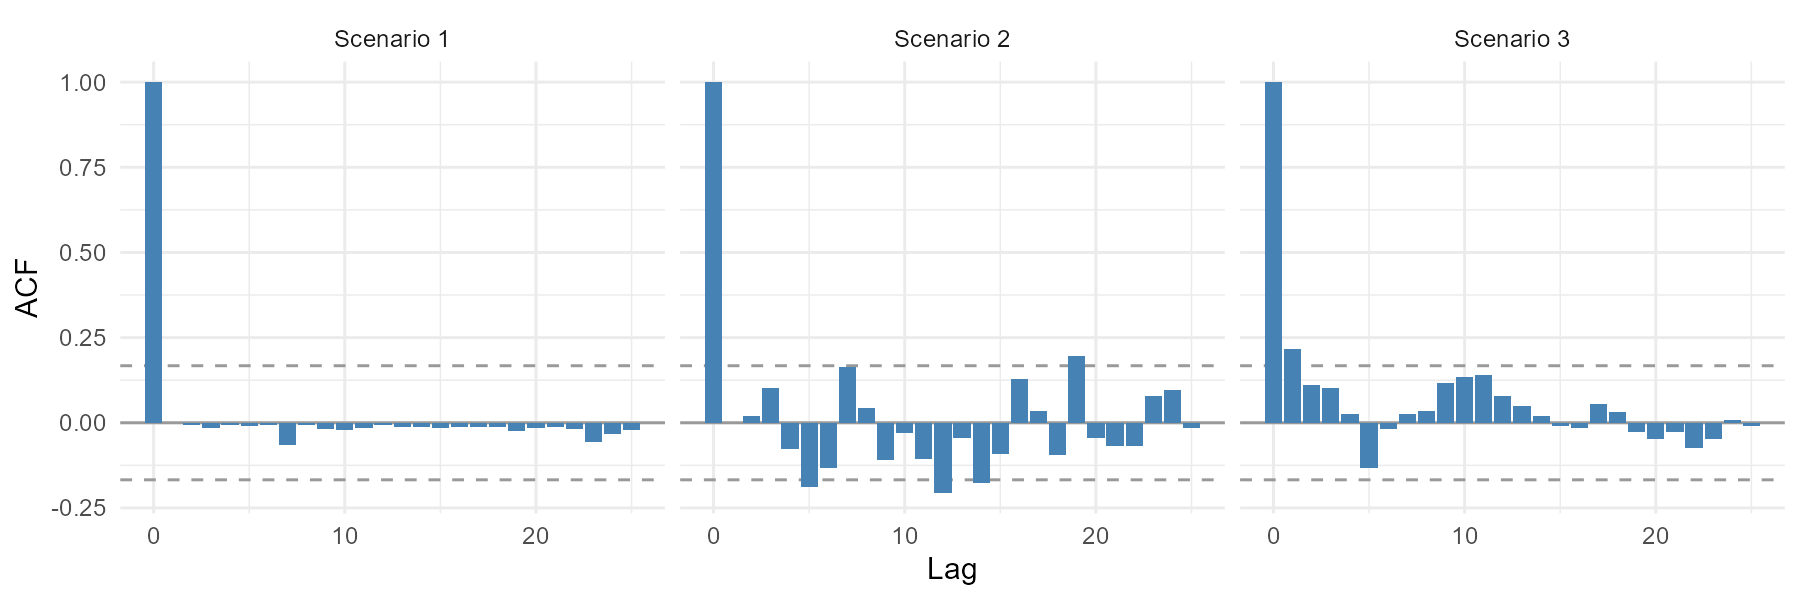
\includegraphics[width=0.92\linewidth]{figs/sma-fig-res-acf-1.png}
  \caption{sma fig res acf 1}
  \label{fig:robustness-sma-fig-res-acf-1}
\end{figure}



\subsection{Best Assessment Versus Ensemble}

If the estimates from pre-specified alternative models remain within the uncertainty
intervals of the reference model for the management quantities of interest, a best
assessment may be adequate for advice. If model sensitivity is larger than estimation
uncertainty, especially for limit tail probabilities or target central tendencies, advice is
model-dependent and should be reported using a scenario set or ensemble.

% Best-assessment versus ensemble comparison (MVLN).

% Reference scenario: Scenario-1; MVLN Monte Carlo draws = 500 per scenario.

\begin{table}

\caption{\label{tab:robustness-mvln-ensemble}MVLN terminal status and tail probabilities (year 2023). Compare estimation uncertainty (reference) with structural sensitivity scenarios.}
\centering
\begin{tabular}[t]{llrrrrrrrrrr}
\toprule
  & scenario & terminal\_year & stock\_median & stock\_p05 & stock\_p95 & harvest\_median & harvest\_p05 & harvest\_p95 & p\_overfished & p\_overfishing & weight\\
\midrule
Scenario-1 & Scenario-1 & 2023 & 1.05 & 0.867 & 1.32 & 24.3 & 21.0 & 27.9 & 0.326 & 1 & 0.333\\
Scenario-2 & Scenario-2 & 2023 & 1.06 & 0.926 & 1.22 & 25.4 & 23.1 & 28.1 & 0.220 & 1 & 0.333\\
Scenario-3 & Scenario-3 & 2023 & 1.16 & 0.938 & 1.42 & 43.3 & 35.5 & 52.7 & 0.112 & 1 & 0.333\\
\bottomrule
\end{tabular}
\end{table}

\begin{table}

\caption{\label{tab:robustness-ensemble-weight-comparison}Ensemble weight comparison by scenario: (i) equal weights; (ii) ICES-style Akaike weights $w_i \propto \exp(-\Delta\mathrm{AIC}/2)$ from total SS3 negative log-likelihood (comparable models); (iii) CVindexmase; (iv) CVindexrho (hindcast skill from retrospective peels; Scenarios 2--3 only until LOO CPUE is collected).}
\centering
\begin{tabular}[t]{lrrrr}
\toprule
scenario & w\_equal & w\_ices & w\_cvindexmase & w\_cvindexrho\\
\midrule
Scenario-1 & 0.3333 & 0 & NA & NA\\
Scenario-2 & 0.3333 & 1 & 1 & 0.6667\\
Scenario-3 & 0.3333 & 0 & 0 & 0.3333\\
\bottomrule
\end{tabular}
\end{table}

\begin{figure}[H]
  \centering
  \includegraphics[width=0.92\linewidth]{appendices/figs/robustness/mvln-kobe-terminal.png}
  \caption{Terminal-year Kobe-style comparison of MVLN draws: reference (Scenario-1) vs structural sensitivity scenarios.}
  \label{fig:robustness-mvln-kobe}
\end{figure}

\begin{figure}[H]
  \centering
  \includegraphics[width=0.92\linewidth]{appendices/figs/robustness/mvln-terminal-compare.png}
  \caption{Terminal MVLN medians and 5--95\% intervals for SSB/BMSY and F/FMSY by scenario.}
  \label{fig:robustness-mvln-terminal}
\end{figure}

\begin{figure}[H]
  \centering
  \includegraphics[width=0.92\linewidth]{appendices/figs/robustness/mvln-status-ts.png}
  \caption{Recent-year MVLN status trajectories with 5--95\% intervals by scenario.}
  \label{fig:robustness-mvln-ts}
\end{figure}



\subsection{Interpretation}

State which advice quantities are robust, which are model-dependent, and whether the
case study should be presented as a best assessment, a screened scenario set, an ensemble,
or an MSE operating-model set.

% Case-specific robustness interpretation.
% State which advice quantities are robust, which are model-dependent,
% and whether reporting should use a best assessment, screened scenario set, or ensemble.




\bibliographystyle{plainnat}
\bibliography{refs.bib}

\end{document}
